\documentclass{bioinfo}
\usepackage{url}

\usepackage[british,english]{babel}
\usepackage{mathpazo}
\usepackage[T1]{fontenc}
% \usepackage[latin9]{inputenc}
\usepackage{float}
\usepackage{amsmath}
\usepackage{graphicx}
\usepackage{setspace}
\usepackage{amssymb}
\usepackage{natbib}
\usepackage[title]{appendix}
\usepackage{siunitx}
\usepackage{chngcntr}
\usepackage{algorithmic}
\renewcommand{\algorithmicrequire}{\textbf{Input:}}
\renewcommand{\algorithmicensure}{\textbf{Output:}}

\makeatletter
\newfloat{algorithm}{H}{loa}[section]
\floatname{algorithm}{Algorithm}
\counterwithout{algorithm}{algorithm}
\def\argmin{\mathop{\operator@font arg\,min}} 
\def\argmax{\mathop{\operator@font arg\,max}} 
\makeatother

\copyrightyear{}
\pubyear{}

\begin{document}
\firstpage{1}

\title[QuickBundles]{QuickBundles, a method for tractography simplification}

\author[Garyfallidis, Brett, Correia, Williams and
Nimmo-Smith]{Eleftherios~Garyfallidis\,$^{1,3,*}$, Matthew~Brett\,$^{2}$,
  Marta~Morgado~Correia\,$^{3}$, Guy~B.~Williams\,$^{4}$ and
  Ian~Nimmo-Smith\,$^{3}$\footnote{to whom correspondence should be
    addressed. e-mail: garyfallidis@gmail.com}}

\address{\,$^{1}$Wolfson College, University of Cambridge, Cambridge, UK\\
  \,$^{2}$University of California, Henry H. Wheeler, Jr. Brain Imaging Center, Berkeley, CA.\\
  \,$^{3}$MRC Cognition and Brain Sciences Unit, Cambridge, UK.\\
  \,$^{4}$Wolfson Brain Imaging Centre, University of Cambridge,
  Cambridge, UK.}


\history{}

\editor{}

\maketitle

\begin{abstract}
\noindent
Diffusion MR white matter tractographies are very large data sets which
are hard to visualize, interact with, and interpret in a clinically
acceptable time scale, despite numerous proposed approaches. As a
solution we present a simple, compact, tailor-made clustering algorithm,
QuickBundles (QB), that overcomes the complexity of these large data
sets and provides informative clusters in seconds. Each QB cluster can
be represented by a single centroid streamline; collectively these
centroid streamlines can be taken as an effective representation of the
tractography. We provide a number of tests to show how the QB reduction
has good consistency and robustness. We show how the QB reduction can
help in the search for similarities across several subjects.

% We demonstrate how these centroid streamlines can be used
% as input to clustering algorithms of higher order complexity which
% currently cannot be implemented on full data sets.
% We also show the
% further potential of QB to find landmarks, create atlases, compare and
% register tractographies

\section{Keywords:} Tractography, Diffusion MRI, Fiber clustering, White
matter Segmentation, Dimensionality Reduction, Clustering algorithms, DTI.

\end{abstract}


\section{Introduction}

Following the acquisition of diffusion MR scans, processes of
reconstruction and integration are performed to create a tractography: a
data set composed of streamlines, which are sequences of points in 3D
space. Irrespective of the types of reconstruction and integration, a
tractography can contain a very large number of streamlines (up to
$10^6$) depending principally on the number of seed points used to
generate the tractography but also on how the tractography propagation 
algorithm handles voxels with underlying fiber crossings.

\begin{figure*}[htp]
\centerline{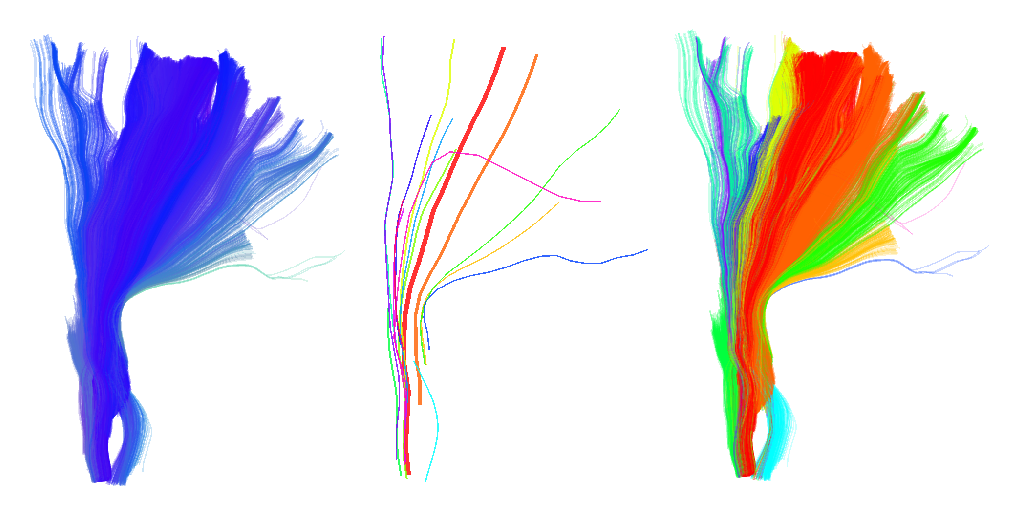
\includegraphics[width=160mm]{Figures/Fig_4_cst_simplification_relabeled_triple.eps}}
    % \par\end{centering}
\caption{Part of the CST bundle (left in blue) consisting of \num{11041}
  streamlines. At first glance it looks as though all streamlines have a
  similar shape, and possibly converge towards the bottom, and fan out
  towards the top. However, this is a misreading caused by the opaque
  density when all the streamlines are visualised.  QB can help us see
  the finer structure of the bundle and identify its elements. In the
  middle we see the 16 QB centroid streamlines of the CST. We can now
  clearly observe that several parts which looked homogeneous are
  actually broken bundles or bundles with rather different shapes. On
  the right panel we see the streamlines coloured according to their
  cluster label. The distance threshold used here was
  $10$~mm. \label{Flo:cst_pbc}}
\end{figure*}


The size of these tractographies makes them difficult to interpret and
visualize. A clustering of some kind seems to be an obvious route to
simplify the complexity of these data sets and provide a useful
segmentation.  As a result, during the last 10 years there have been
numerous efforts by many researchers to address both unsupervised and
supervised learning problems of brain tractography. 
% Though these studies
% do provide many useful ideas, all these methods suffer ultimately from
% lack of practical efficiency.
% During the last $10$ years there have been numerous efforts from many
% researchers to address the unsupervised and supervised learning problems
% of brain tractography. 
As far as we know all these methods suffer from low efficiency, however 
they provide many useful ideas which we describe in this section.

Tractography clustering algorithms are rarely compared in the
literature.  In this regard, \citet{moberts2005evaluation} is an
exception. \citeauthor{moberts2005evaluation} evaluated different
popular hierarchical clustering methods including a less common one,
shared nearest neighbor (SNN), against a gold standard segmentation by
physicians. The authors concluded that single-link clustering with mean
average distance was the method which performed best.

\citet{wang2010tractography} proposed a nonparametric Bayesian framework
using hierarchical Dirichlet processes mixture model (HDPM). This is one
of the very few methods not based on distances. In this work a
streamline is modeled as a discrete distribution over a codebook of
discretized orientations and voxel regions. The authors explain that
calculating pairwise distances is very time consuming and therefore they
avoid using them. Their approach automatically learns the number of
clusters from data with Dirichlet processes priors but it is still not
efficient enough for real time operation. A disadvantage of this method
is that the priors do not originate from anatomical knowledge.

\citet{Visser2010} used hierarchical clustering and fuzzy c-means
together with recombination of subsets of the same tractography to
reduce the effect of the large data sets on the distance matrix based on
the MDF distance (see section~\ref{sub:track-distances})
\citep{EGMB10}. An interesting result with this method was that they
could automatically find the different sub-bundles of the Arcuate
Fasciculus region in accordance with the supervised labeling described
in \citet{catani2005perisylvian}. In common with \citet{Visser2010} the
algorithm that we present in this paper also uses the minimum average
flip (MDF) distance function as a measure of distance between
streamlines. \citet{gerig2004analysis} also used hierarchical clustering
with a symmetrised version of two closest point Hausdorff-type
distances.
% $\mathrm{MA}\mathrm{M}_{\mathrm{avg}}$ and
% $\mathrm{MA}\mathrm{M}_{\mathrm{max}}$ (Hausdorff). 
However, they tested
their method only with two bundles: Uncinate Fasciculus and the
Corticospinal Tract.

\citet{Guevara2010} combined a great number of different algorithms from
hierarchical clustering to 3D watershed on streamline extremities.  They
first divided the tractography into left-right hemisphere,
inter-hemispheric and cerebellum subsets. They then create further
subsets of different streamline length, use hierarchical clustering
based on the random voxel parcels, use watershed over extremities and
finally use hierarchical clustering to merge the different sub-bundles
using the Hausdorff distance (see section
\ref{sub:track-distances}). This work stressed the need to divide the
data set between shorter and longer streamlines.

\citet{Tsai2007} used a combination of cluster methods based on minimum
spanning trees, locally linear embedding and k-means.  They were able to
incorporate both local and global structures by changing a few
parameters. The main advantage of this method was that it showed a way
to merge a long chain of neighbouring structures into one cluster.

\citet*{zhang2005dti} used an agglomerative hierarchical clustering
using the same distance as in \citet{zhang2003visualizing} and later in
\citet{zhang2008identifying} combined distance-based single linkage
hierarchical clustering with expert labeling of specific
bundles. 

\citet{zvitia2008adaptive, Zvitia2010} used adaptive mean shift. This is
a clustering algorithm which finds automatically the number of clusters
for example in contrast with k-means that the user needs to prespecify
the number of clusters.  They also used this approach for direct
registration of tractographies but only with tractographies from the
same subject.

\citet{ElKouby2005} created a ROI-based connectivity matrix where the
$i,j$th entry of the matrix holds the number of streamlines which
connect $ROI_{i}$ to $ROI_{j}$. K-means was used afterwards on the rows
of the matrix to cluster the streamlines. 
% This technique can be used for
% clustering bundles across subjects.

\citet{brun2004clustering} used the mean and covariance of the
streamline as the feature space and normalized cuts based on a graph
theoretic approach for the segmentation. \citet{Ding2003a} used
k-nearest neighbours, another agglomerative approach, applied to
corresponding streamline segments. \citet{corouge2004towards} used
different types of streamline distances, e.g. Hausdorff distances, and
higher order geometric properties such as torsion and curvature, and in
\citet{Corouge2004} and \citet{Corouge2006} used Generalized Procrustes
Analysis and Principal Components Analysis (PCA) to analyze the shape of
bundles.

\citet{ODonnell_IEEETMI07} created a tractographic atlas using spectral
embedding and expert anatomical labeling. They then automatically
segmented using spectral clustering and expressed the streamlines as
points in the embedded space to the closest existing atlas clusters. The
full affinity matrix was too big to compute therefore they used the
Nystrom approximation: working on a subset and avoid generating the
complete affinity/distance matrix. Later in \citet{o2009tract} they
performed group analysis on pre-specified bundles.


\citet{Maddah_MICCA2005} used B-spline representations of streamlines
referenced to an atlas, and then the streamlines were clustered based on
the labeled atlas. Later \citet{maddah2006statistical} using a similar
streamline representation (quintic B-splines) calculated a model for
each bundle as the average and standard deviation of that parametric
representation. In this way they created an atlas which is used as a
prior for expectation-maximization (EM) clustering of the Corpus
Callosum streamlines into Witelson subdivisions \citet{witelson1989hand}
using population averages. Later in \citet{Maddah_IEEEBI2008} showed
that it is possible to combine spatial priors with metrics for the shape
of the streamlines in order to guide the clustering process.

\citet{jonasson2005fiber} created a large $N\times N$ co-occurrence
matrix, where $N$ is the number of the fibers to cluster.  The
co-occurrence matrix contained the number of times that two fibers share
the same voxel. They then used spectral clustering.
\citet{jianu2009exploring} presented a new method for visualizing and
navigating through tractography data combining dendrograms from
hierarchical clustering along with 3D- and 2D-embeddings using the
approximation that \citet{chalmers1996linear} introduced for the
technique of \citet{eades1984heuristic}.

\citet{Durrleman2009} introduced electrical current models of fibre
bundles where a fibre is seen as a set of wires sending information in
one direction at constant rate. Currents have good diffeomorphic
properties and can be used for registration of bundles as shown in
\citet{Durrleman2009} and later in \citet{durrleman2010registration}.
This methodology does not impose point-to-point or fibre-to-fibre
correspondences, however it is sensitive to fibre density and
orientation of the bundles and it is computationally expensive.

\citet*{leemans17new} used affinity propagation to cluster the
fronto-occipital fibres, Cingulum and Arcuate Fasciculus after reducing
the complexity of the data sets using additional frontal and occipital
boolean masks on the right cerebrum. Results however were shown on a
very small part of the entire tractography where clustering is a much
easier problem.  Later \citet{malcolm2009filtered} used affinity
propagation to cluster a full brain tractography created using filtered
tractography and suggested that affinity propagation is not suitable for
group clustering of tractographies.

\citet{ziyan2009consistency} introduced a probabilistic registration and
clustering algorithm based on expectation-maximization (EM) which
creates a sharper atlas from a set of subjects based on three bundles:
Corpus Callosum, Cingulum and Fornix. This work used an initial
spectral clustering \citep{ODonnell_IEEETMI07} to label the bundles and
then updated these labels iteratively while performing bundle-wise
registration using a poly-affine framework \citet{Arsigny2009}.

Often it is useful to have some anatomical guidelines in order to add
prior information to the automated learning process. Protocols to
manually label $11$ major white matter tracts were described in
\citet{Wakana2007NeuroImage} using ROIs to include or exclude
streamlines generated by deterministic tractography.
\citet{Hua2008NeuroImage} used regions of interest together with
probabilistic tractography in order to create probability maps of known
fibre bundles.

From this short overview we observe two main trends in the literature.
The first and most common one makes use of streamline distances and
calculates distance matrices. The most prevailing approaches here for
deciphering the distance matrix are with Hierarchical and Spectral
Clustering which are applied only on random subsets of the initial
tractography. For example, \citet{ODonnell_IEEETMI07} used only
\num{10000} streamlines (~10\% of the initial tractography) and
\citet{Visser2010} used recombinations of \num{10000} streamlines. The
second trend, and the less common, favours avoiding streamline distances
because the computation of the distance matrix is memory intensive. In
this case using Dirichlet Processes or Currents or Connectivity based
parcellation seem to be some viable solutions. For further recent
overviews see \citet{ODonnell_IEEETMI07} and
\citet{wang2010tractography}.

All the same, if clustering is to be used in clinical practice or to
make neuroscientists' analysis more efficient and practical we need
algorithms that can provide useful clusters and cluster descriptors in
acceptable time. None of the papers covered in this literature review
provide a solution for this issue of efficiency and most of the methods
would require from many hours to many days to run on a standard sized
data set.

% The method we propose in this document can provide a solution
% to this problem and it is an extensive update of our preliminary work
% described in \citet{EGMB10}.

Most authors agree that unsupervised learning with tractographies is a
difficult problem as the data sets are very large, dense, cluttered with
noisy streamlines which could have no anatomic relevance, and the actual
anatomical bundles are interwoven in a complicated way in several brain regions.
% Furthermore, we note that there is wide disagreement on the
% number of clusters (from 10 to 60). Because of the difficulty of the
% problem an international contest was also organized by SchLab in
% Pittsburgh University (PBC Brain Connectivity Challenge - IEEE ICDM) in
% $2009$. The competition did not identify any directly viable
% solutions. 
We think that in order to find larger anatomical clusters a significant
amount of anatomical prior knowledge needs to be introduced in a way
that is not yet established.

For these reasons we propose to take a step back to first get the
tractography into a suitable form for working with neuroanatomists to
capture this prior knowledge. The clustering that we propose
concentrates on reducing the complexity of the data rather than finding
bundles with hopefully anatomical relevance. We believe this step is
more useful at this stage of tractography analysis research.

Most of these proposed tractography clustering algorithms are very slow
and many need to calculate a matrix of inter-streamline distances of
size $\mathcal{O}(N^2)$.  This number of computations puts a very heavy
load on clustering algorithms, making them hard to use for everyday
analysis as it is difficult to compute all these distances or store them
in memory. For the same reason, no current algorithm is practical for
real time clustering on a large number of streamlines -- despite the
innovations in tractography clustering algorithms there is no parallel
uptake by anatomists or clinicians. The heavy computational demands of
clustering add a further overhead to the use of tractography for
clinical applications but also put a barrier on understanding and
interpreting the quality of diffusion MR data sets. Moreover methods
described as `automatic' in reality require significant intervention
using neuroanatomical knowledge.

In fact tractographies have high levels of redundancy with very many
quite similar streamlines. Our approach is to take advantage of this to
reduce the size and dimensionality of the datasets as a precursor for
higher complexity classification and/or input from experts. To address
thes key issues of time and space we present a stable, generally linear
time clustering algorithm that can generate meaningful clusters of
streamlines in seconds with minimum memory consumption. Our approach is
extremely straightforward and we do not need to calculate all pairwise
distances unlike most existing methods. Furthermore we can update our
clustering online. In this way we can overcome the previous barriers of
space and time.

We show that we can generate these clusters \textasciitilde1000 times
faster than any other available method before even applying further
acceleration through parallel processing, and that it can be used to
cluster from a few hundred to many millions of streamlines.

% Moreover our new algorithm leads to many valuable additional results. QB
% can either be used on its own to explore the neuroanatomy directly, or
% it can be used as a precursor tool which reduces the dimensionality of
% the data, which can then be used as an input to other algorithms of
% higher order complexity, resulting in their greater efficiency. Beyond
% the use of this algorithm to simplify tractographies, we show how it can
% help find landmarks, create atlases, and compare and register
% tractographies.

% \subsection{Focus}

% Many published methods on tractography segmentation - some evidence of
% lengthy computation time - because of size of datasets on top of
% complexity of segmentation methods - lack of evidence that methods have
% been taken up and used for practical problems - ‘automatic’
% classification in reality requires significant intervention by
% neuroanatomists - data sets have high redundancy with many rather
% similar tracks - our approach is to reduce the size and dimensionality
% of the datasets by QB as a precursor for higher complexity
% classification and/or input from experts. We provide a number of tests
% to show how the QB reduction has good consistency, robustness etc. We
% show one application involving multiple subjects - to look at the
% correspondence problem and hint at the power of the QB approach.

% Data reduction - preprocessing - unsupervised - automatic. No claims for
% anatomical segmentation.

There is no current unsupervised anatomical segmentation method that can
have general usability without expert knowledge
integration. Nonetheless, neuroanatomists often disagree on definition
of major structures or on which streamlines correspond to actual tracts
\citep{schmahmann2009fiber, makris2005segmentation,
frey2008dissociating,catani2005perisylvian,
moriBook, fernandez2012high, verstynen2011vivo}.
%\textbf{well there's the old 'extreme capsule fibre system' (Schmahmann, Pandya, Makris, Petrides) vs. 'fronto-occipital fasciculus' (Catani, Wakana, Mori, (i.e JHU peeps)). I'm not sure so many people disagree on names so much as disagree on the appropriate names to use for tractography since tractography often can't distinguish between small bundles e.g. SLF I-III and IV (arcuate). Some people would prefer to just say SLF for tractography or temporal part of SLF(that's Wakana et al. 2007, 2004). I think there may possibly be some overlap between the superior occipitofrontal fasciculus and one of SLF I-III not 100\% sure but Thiebaut de Schotten (e.g. 2008) \& Catani use SOF terminology some people use the proper names for the corpus callosum segments whereas other people just say something like anterior, mid, posterior}. 
What we propose is to create a method that simplifies the tractography
at the level where such distinctions are not an issue (see
Fig.~\ref{Flo:cst_pbc}).

\begin{methods}

\section{Methods and Materials}

\subsection{\label{sub:track-distances}Streamline distances and preprocessing}

A wide range of approaches have been taken in the literature for
representing or coding for tractographies~\citep{Guevara2010,
  chung2010cosine}. The approach we have taken with streamline coding
has gone in parallel with the selection of appropriate functions for
inter-streamline distances.  Numerous inter-streamline distance
functions have been proposed~\citep{Ding2003, MaddahIPMI2007,
  zhang2005dti}. The most common is the Hausdorff distance~\citep[and
many other studies]{corouge2004towards}. There are two primary
disadvantages of this function: it ignores the sequential nature of the
streamlines and treats each streamline simply as a cloud of points, and
its computation requires every point on the first streamline to be
compared with every point on the second streamline, and vice versa. Thus
the Hausdorff distance requires the calculation $\mathcal{O}(KL)$
inter-point distances when comparing streamlines of $K$ and $L$ points.

\begin{figure}
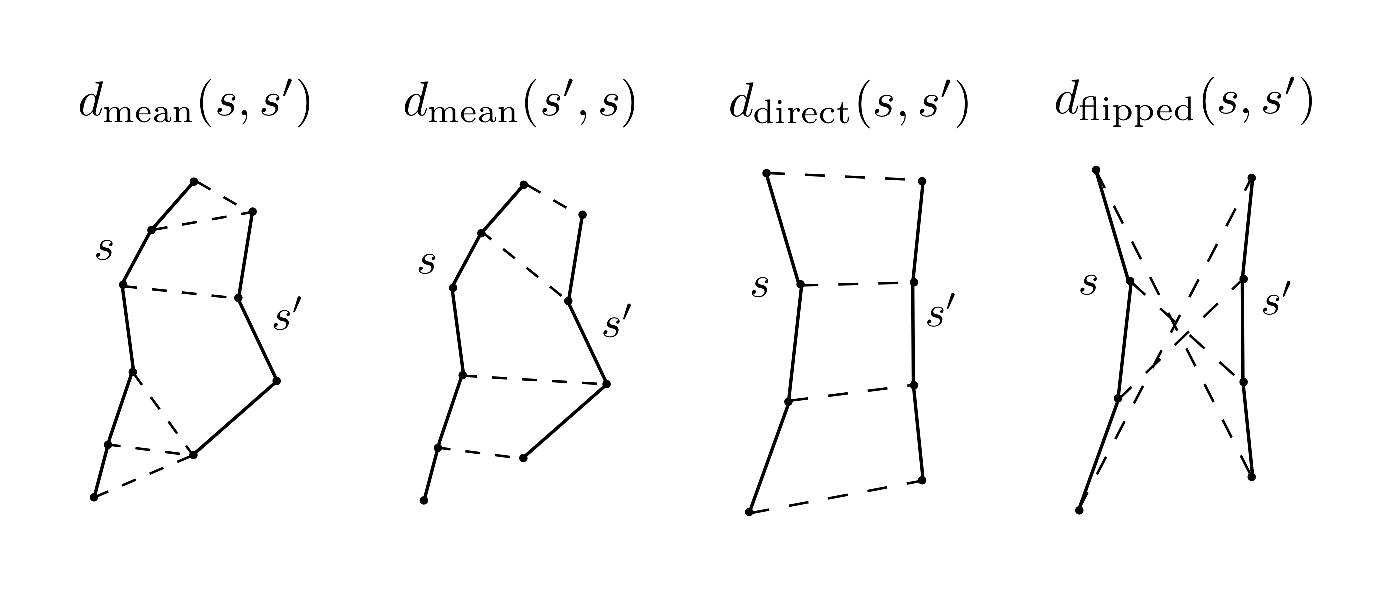
\includegraphics[scale=0.35]{Figures/Fig_2_distances2}
\centering{}
\caption{The principal distance used in this work is minimum average
  direct flip distance
  $\textrm{MDF}=\min(d_{\textrm{direct}},d_{\textrm{flipped}})$ which is
  a symmetric distance function that can deal with the streamline
  bi-directionality problem; it works on streamlines which have the same
  number of points.  Another distance we use is the mean average
  distance which is again symmetric but does not require the streamlines
  to have the same number of points: $\textrm{MAM}_{\textrm{mean}} =
  (d_{mean}(s, s') + d_{mean}(s',s))/2$ (see Eq.~(\ref{eq:mean_average_distance})).  In this
  figure the components of both distances are shown; the streamlines are
  drawn with solid lines, and then with dashed lines we connect the
  pairs of points of the two streamlines whose distances contribute to
  the overall metric. Note that we cannot calculate the $\textrm{MDF}$
  between the streamlines on the left of the figure because they have
  different numbers of points.
  \label{Flo:Distances_used}}
\end{figure}


For these reasons we have opted to use a rather simpler symmetric
distance function~\citep{EGMB10, Visser2010} which we call the minimum
average direct-flip (MDF) distance, see
Eq.~(\ref{eq:direct_flip_distance}). MDF can be applied only when both
streamlines have the same number of points, see
Fig.~\ref{Flo:Distances_used}. Therefore we assume that an initial
downsampling of streamlines has been implemented, where all segments on
a streamline have approximately the same length, and all streamlines
have the same number of points $K$, which are much fewer than the number
of points in the typical raw streamline. We make this assumption in what
follows.

As it has no preferred orientation, a streamline $s=[s_1, s_2, \ldots, s_K]$ is equivalent to
two ordered polylines: $s = (s_1, s_2, \ldots, s_K)$ in $\mathbb{R}^3$
and its flipped version $s^F = (s_K, s_{K-1}, \ldots, s_1)$.  With this
notation the direct, flipped and MDF distances are defined as follows:
\begin{eqnarray}
  d_{\textrm{direct}}(s, t) = d(s, t) & = & \frac{1}{K}\sum_{i=1}^{K}|s_{i}-t_{i}|,\nonumber\\
  d_{\textrm{flipped}}(s, t) & = & d(s,t^F) = d(s^F,t),\nonumber\\
  \textrm{MDF}(s, t) & = & \min(d_{\textrm{direct}}(s, t), d_{\textrm{flipped}}(s, t))\label{eq:direct_flip_distance}.
\end{eqnarray}
\noindent
Here $|x-y|$ denotes the euclidean distance between two points $x$ and
$y$. The direct distance $d_{\mathrm{direct}}(s, t)$ between two
streamlines $s$, and $t$ is the mean of the euclidean distances between
corresponding points. Clearly the MDF distance between two streamlines
of $K$ points requires the calculation of just $2K$ inter-point
distances.

The MDF distance is in fact a metric on the space of streamlines.
Obviously MDF distances are non-negative, are zero if and only if the
two streamlines are identical, and symmetrical.  The triangle inequality
is established as follows. Let $s$, $t$ and $u$ be three streamlines
and assume, without loss of generality, that $d(s,t)$ and $d(t,u)$ actually
minimise the corresponding MDF distances $\mathrm{MDF}(s,t)$ and
$\mathrm{MDF}(t,u)$. (If not, we replace e.g.~$t$ by $t^F$) Then
$\mathrm{MDF}(s, t) + \mathrm{MDF}(t, u) = d(s, t) + d(t, u) \ge d(s,
u)$ (by the triangle inequality for the euclidean distance) $ \ge
\min(d(s,u), d(s, u^F)) = \mathrm{MDF}(s, u)$.

\begin{figure}
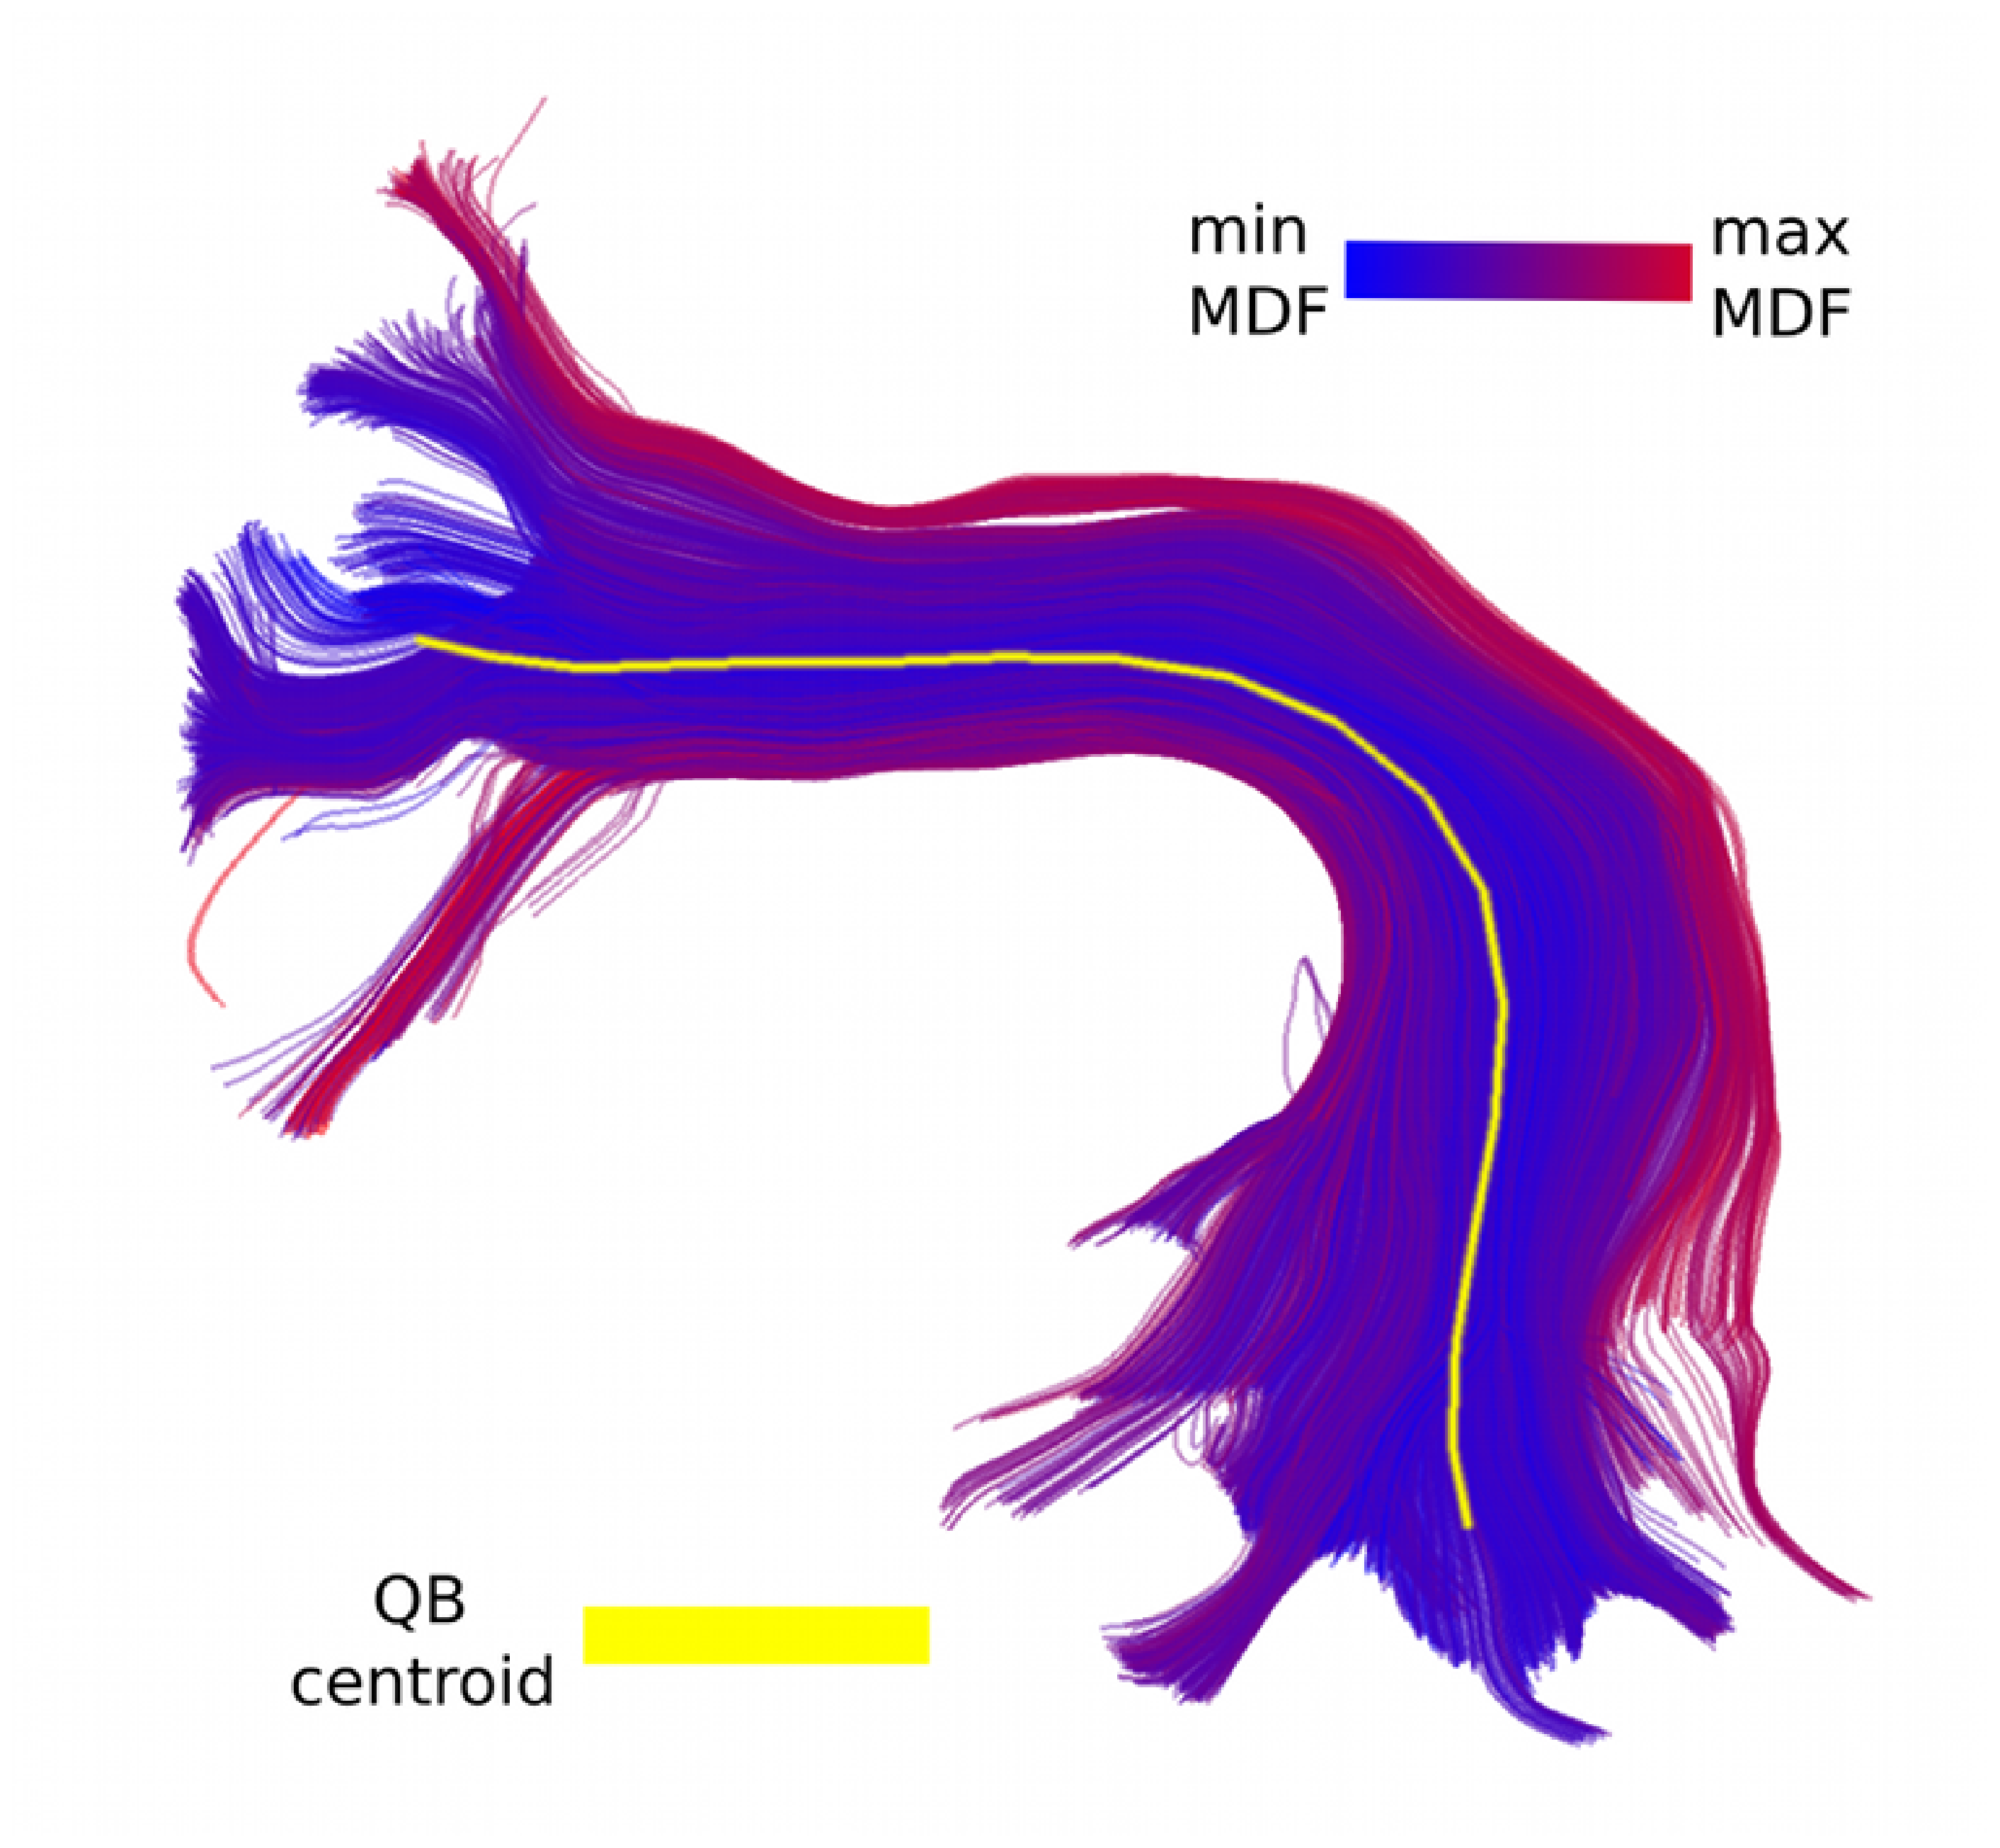
\includegraphics[scale=0.15]{Figures/Fig_11_MDF_arcuate}
\centering{}
\caption{Color coding shows MDF distances from QB centroid to every other track in the bundle.\label{Flo:MDF_arcuate}}
\end{figure}


The main advantages of the MDF distance are that it is fast to compute,
it takes account of streamline direction issues through consideration of
both direct and flipped streamlines, and that its behaviour is easy to
understand (see Fig.~\ref{Flo:MDF_arcuate}), from the simplest case of
parallel equi-length streamlines to the most complicated with very
divergent streamline.

Another advantage of the MDF distance function is that it separates
short streamlines from long streamlines; a streamline $s$ that is a
portion of a streamline $s'$ will be relatively poorly matched on MDF to
$s'$. This is consistent with our proposed approach to leave decisions
about the status of short versus long streamlines till after applying a
clustering. At this later stage one can determine whether there are
several similar short streamlines -- perhaps reflecting a damaged fiber
tract -- or localised noise if there are only a few similar streamlines.

A further important advantage of having streamlines with the same number
of points is that we can easily do pairwise calculations on them; for
example add two or more streamlines together to create a new average
streamline. We will see in the next section how streamline addition is a
key property that we exploit in the QB clustering algorithm.

Care needs to be given to choosing the number of points required in a
streamline (streamline downsampling). We always keep the endpoints
intact and then downsample into segments of equal lengths. One
consequence of short streamlines having the same number of points as
long streamlines is that more of the curvature information from the long
streamlines is lost relative to the short streamlines i.e. the short
streamlines will have higher resolution.  We found empirically that this
is not an important issue and that for clustering purposes even
downsampling to only $K=3$ points in total can be useful
\citep{EGMB10}. Depending on the application, more or fewer points can
be used. In the results presented we often use $K=12$ which achieves a
good trade-off between streamline resolution and dimensionality
reduction.

In some later stages in the analysis of tractographies. e.g.~for merging
clusters, we find a use for Hausdorff-type distance functions which for
simplicity we denote as MAM distances -- short for Minimum (or Maximum,
or Mean) Average Minimum distance (MAM). (In this nomenclature the
classical Hausdorff distance is the Maximum Average Minimum distance.)
We mostly use the Mean version of this family, see
Eq.~(\ref{eq:mean_average_distance}) but the others are potentially
useful as they can weight different properties of the streamlines. As
noted above, these distances are slower to compute but they can work
with different number of segments on streamlines; this is useful for
some applications. The equations below show the formulation of these
distances:
\begin{eqnarray}
d_{\textrm{mean}}(s,s') & = & \frac{1}{K_{A}}\sum_{i=1}^{K}d(x_{i},s'),\nonumber \\
d_{\textrm{min}}(s,s') & = & \min_{i=1,...,K}d(x_{i},s'),\qquad\textrm{and}\label{eq:minimum_distance}\\
d_{\textrm{max}}(s,s') & = & \max_{i=1,...,K }d(x_{i},s'),\qquad\textrm{where}\label{eq:maximum distance}\\
d(x,s') & = & \min_{j=1,...,K'}|x-x_{j}'|.\nonumber \\
\textrm{MAM}_{\textrm{min}} & = & \min(d_{\textrm{mean}}(s,s'),d_{\textrm{mean}}(s',s))\label{eq:min_average_distance}\\
\textrm{MAM}_{\textrm{max}} & = & \max(d_{\textrm{mean}}(s,s'),d_{\textrm{mean}}(s',s))\nonumber \\
\textrm{MAM}_{\textrm{mean}} & = & (d_{\textrm{mean}}(s,s')+d_{\textrm{mean}}(s',s))/2\label{eq:mean_average_distance}\end{eqnarray}


\noindent
where the number of points $K$ and $K'$ on the two streamlines are not
necessarily the same. For the same threshold value
$\textrm{MAM}_{\textrm{min}}$, $\textrm{MAM}_{\textrm{max}}$ and
$\textrm{MAM}_{\textrm{mean}}$ will give different results. For example,
$\textrm{MAM}_{\textrm{min}}$ will bring together more short streamlines
with long streamlines than $\textrm{MAM}_{\textrm{max}}$, and
$\textrm{MAM}_{\textrm{mean}}$ will have an in-between effect.  Other
distances than $d(x_{i},s')$ can be used in
Eq.~\ref{eq:minimum_distance} and Eq.~\ref{eq:maximum distance}.
However, we have not investigated them in this work in relation to
clustering algorithms.

\subsection{The QB algorithm\label{sub:QB-description}}

QuickBundles (QB) is a surprisingly simple and very fast algorithm which
can reduce tractography representation to an accessible structure in a
time that is linear in the number of streamlines $N$. QB is an extended
update on our preliminary work~\citet{EGMB10}. By the term
\emph{bundle} we mean here streamlines which are in close proximity
according to a streamline-based distance, therefore, they have similar
spatial and shape characteristics and not necessarily direct
correspondence to neuroanatomical bundles (tracts).

In QB each item, a streamline, is a fixed-length ordered sequence of
points in $\mathbb{R}^{3}$, and QB uses comparison functions and
amalgamations which take account of and preserve this structure.
Moreover each item is either added to an existing cluster on the basis
of the distances between the cluster descriptor of the item and the
descriptors of the current list of clusters. Clusters are held in a list
which is extended according to need. Unlike amalgamation clustering
algorithms such as $k$-means~\citep{steinhaus1956division,
  macqueen1967some} or BIRCH~\citep{zhang1997birch}, there is no
reassignment or updating phase in QB -- once an item is assigned to a
cluster it stays there, and clusters are not amalgamated. QB derives its
speed and efficiency from this idea.

A clustering algorithm needs a measure of distance between two
streamlines, and QB uses a particular distance measure that we call
minimum average direct flip (MDF).  The MDF measure requires that each
streamline be resampled to have $K$ points. We have described the MDF measure
and the resampling in section~\ref{sub:track-distances}.

We index the streamlines with $i = 1 \dots N$ where $s_{i}$ is
the $K\times3$ matrix representing streamline $i$.

QB stores information about clusters in \emph{cluster nodes}.  The
cluster node is defined as $c=(I,h,n)$ where $I$ is the list of
the integer indices $i = 1 \dots N$ of the streamlines in that cluster,
$n$ is the number of streamlines in the cluster, and $h$ is the
\emph{streamline sum}. $h$ is a $K \times3$ matrix which can be
updated online when a streamline is added to a cluster and is equal to:
\begin{equation}
  h=\sum_{i=1}^{n}s_{i}
\end{equation} 
where $s_{i}$ is the $K\times3$ matrix representing streamline $i$,
$\Sigma$ here represents matrix addition, and $n$ is the number of
streamlines in the cluster. One summary of the cluster node is the centroid or
\emph{virtual} streamline $v$ where:
\begin{equation}
  v = h / n
\end{equation}
An example of the QB centroid is presented in Fig.~\ref{Flo:MDF_arcuate}.
%\begin{float}
\begin{algorithm}[h]
%\begin{boxedalgorithmic}
\begin{algorithmic}
\REQUIRE $T=\{s_{1},...,s_{i},...,s_{N}\}$, $\theta$
\ENSURE $C=[c_{1},...,c_{k},...,c_{M}]$ 
\STATE \# create first cluster
\STATE $c_{1} \leftarrow ([1],s_{1},1)$
\STATE $C\leftarrow[c_{1}]$
\STATE $M\leftarrow1$ 
\FOR{$i=2$ to $N$}
	\STATE $\textbf{t}\leftarrow T_{i}$
	\STATE $\texttt{alld}\leftarrow\textbf{infinity}(M)$ \# distance buffer
	\STATE $\texttt{flip}\leftarrow\textbf{zeros}(M)$ \# flipping check buffer
	\FOR{$k=1$ to $M$ }
		\STATE $v\leftarrow c_{k}.h/c_{k}.n$
		\STATE $d\leftarrow d_{\textrm{direct}}(t,v)$
		\STATE $f\leftarrow d_{\textrm{flipped}}(t,v)$
	\STATE \# evaluate MDF
	\IF{$f$ < $d$}
		\STATE $d \leftarrow f$
		\STATE $\texttt{flip}_{k} \leftarrow 1$
	\ENDIF
	\STATE $\texttt{alld}_{k} \leftarrow d$
	\ENDFOR
\STATE $m\leftarrow \min(\texttt{alld})$
\STATE $l\leftarrow \mathrm{arg min}(\texttt{alld})$
\IF{$m < \theta$} 
\STATE \# append to current cluster
	\IF{$\texttt{flip}_{l}$ is $1$} 
		\STATE $c_{l}.h \leftarrow c_{l}.h + t^F)$
	\ELSE
		\STATE $c_{l}.h \leftarrow c_{l}.h + t$
	\ENDIF
	\STATE $c_{l}.n \leftarrow c_{l}.n + 1$
	\STATE \textbf{append}($c_{l}.I$,$i$)
\ELSE 
\STATE \# create new cluster
        \STATE $c_{M+1} \leftarrow ([i],t,1)$
        \STATE \textbf{append}$(C,c_{M+1})$
	\STATE $M\leftarrow M+1$
\ENDIF
\ENDFOR 
\end{algorithmic}
%\end{boxedalgorithmic}
\caption{QuickBundles}
\label{Alg:QuickBundles}
\end{algorithm}

The algorithm proceeds as follows.  At any one step in the algorithm we
have $M$ clusters. Select the first streamline $s_{1}$ and place it in
the first cluster $c_{1}\leftarrow(\{1\}, s_{1},1)$; $M=1$ at this
point.  For each remaining streamline in turn $i = 2 \dots N$: (i)
calculate the MDF distance between streamline $s_{i}$ and the centroid
streamlines $v_{e}$ of all the current clusters $c_{e}$, $e = 1 \dots
M$, where $v$ is defined on the fly as $v=h/n$; (iii) if any of the MDF
values $m_{e}$ are smaller than a distance threshold $\theta$, add
streamline $i$ to the cluster $e$ with the minimum value for $m_{e}$;
$c_{e}=(I,h,n)$, and update $c_{e}\leftarrow(\mathbf{append}(I,i), h+s,
n+1)$; otherwise create a new cluster $c_{M+1}\leftarrow([i],s_{i},1)$,
$M\leftarrow M+1$.

%\subsection{QB Step-by-step\label{sub:QB_step_by_step}}

% \begin{figure*}[t]
% \centering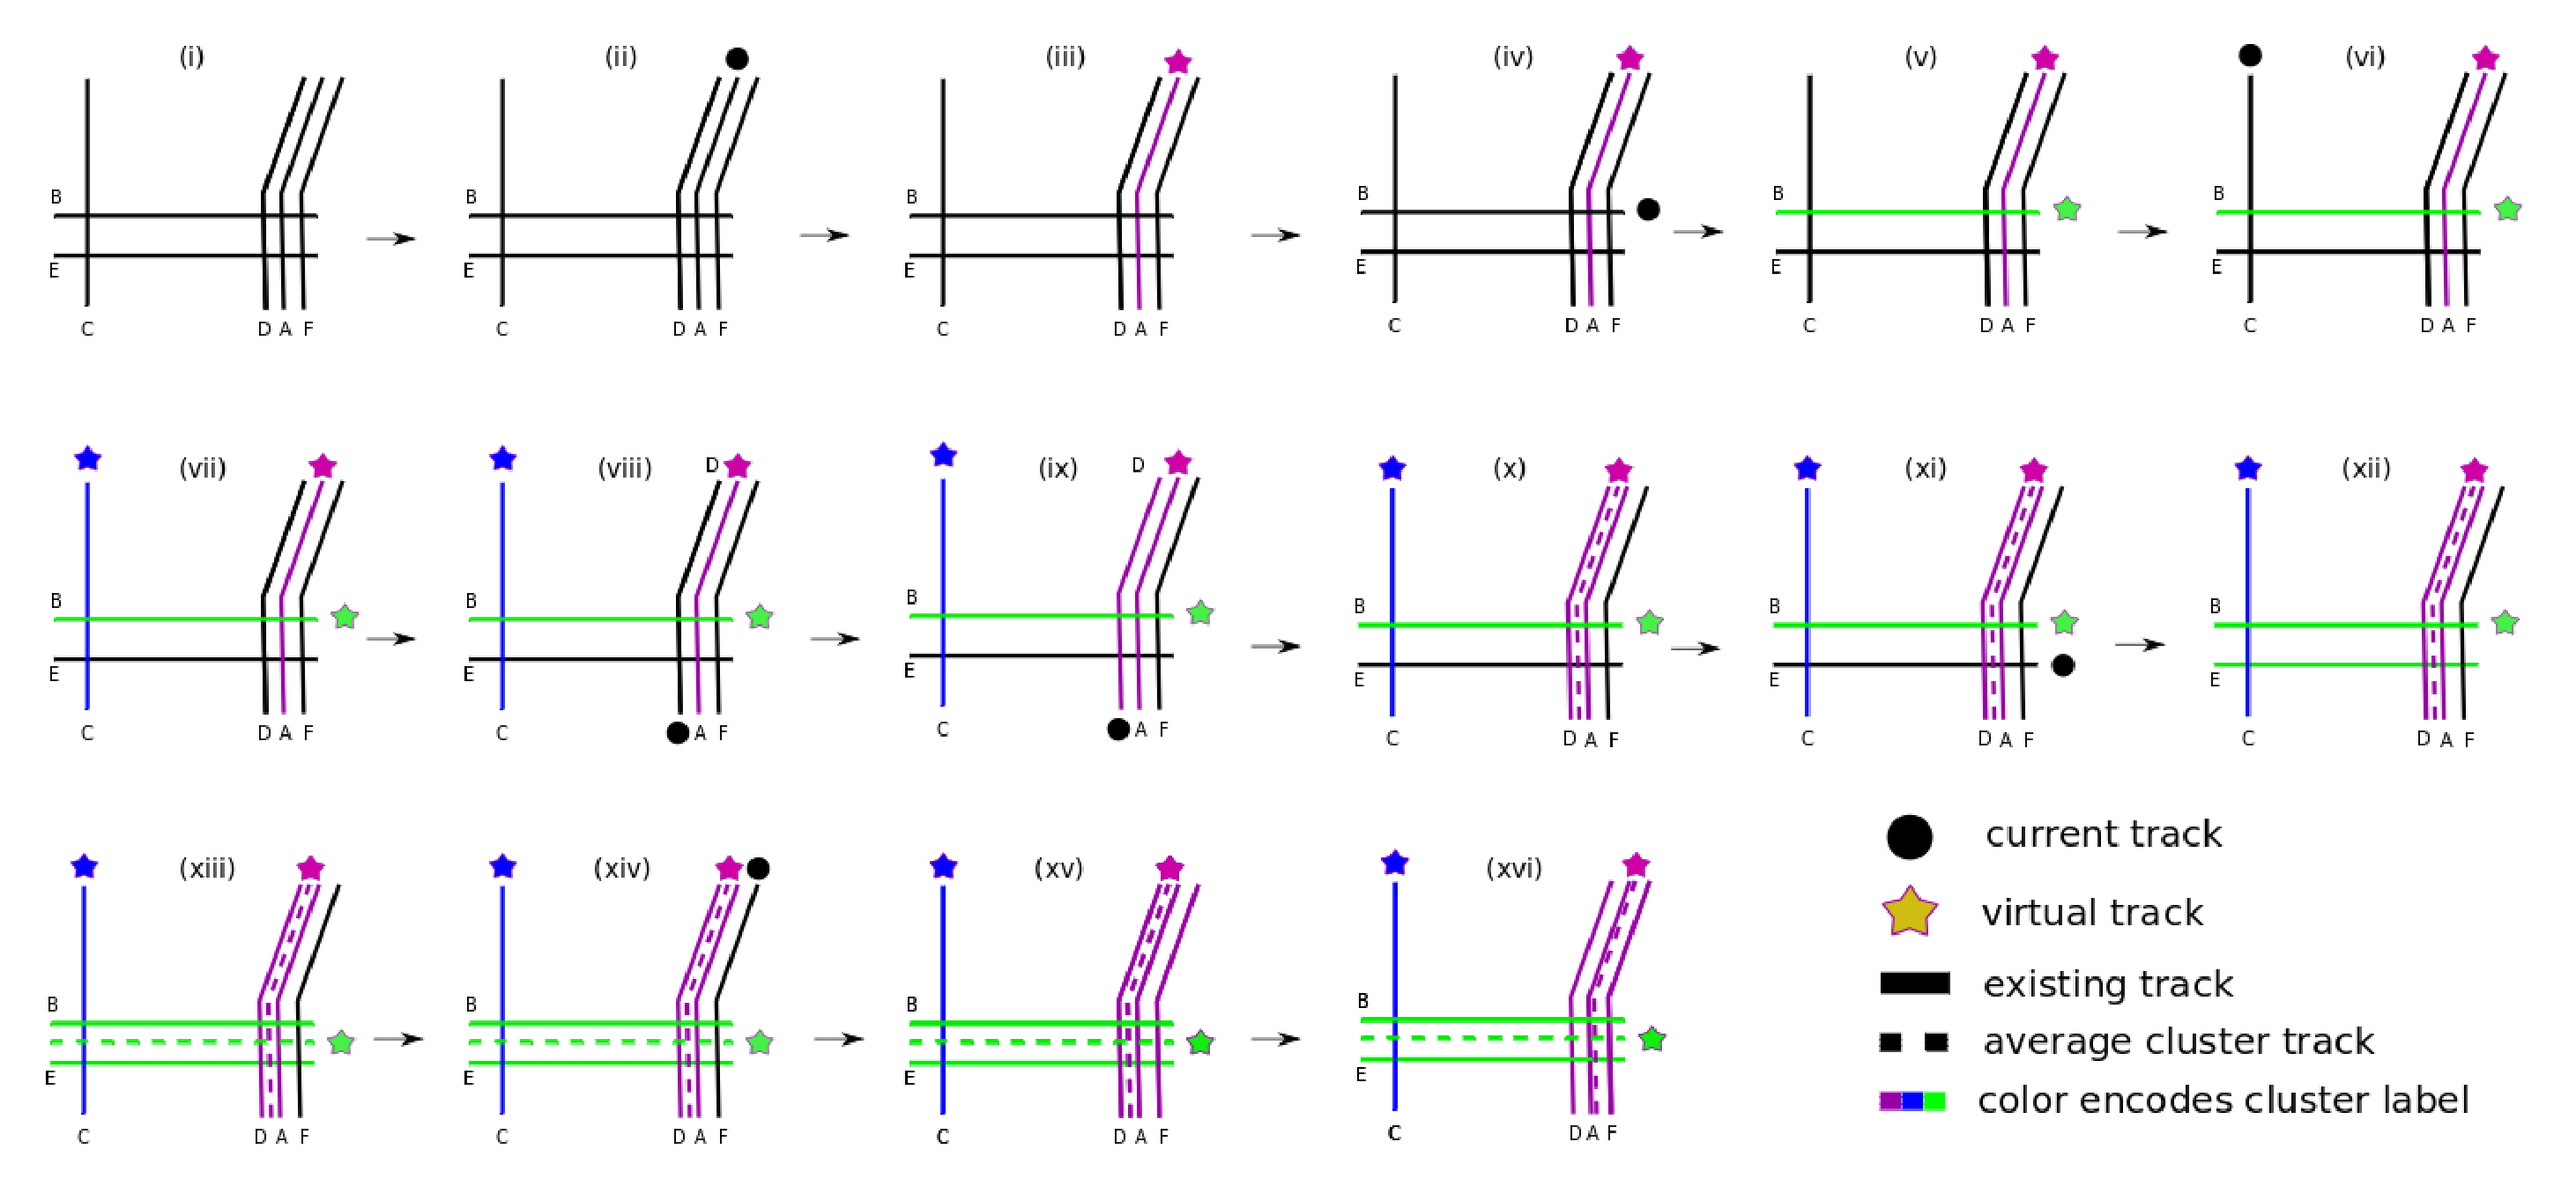
\includegraphics[width=160mm,angle=0]{Figures/Fig_1_QB_algorithm}
% \caption{This is a step-by-step explanation of how QuickBundles proceeds
%   when clustering six streamlines (top left) resulting in three bundles
%   (blue, red and green, bottom right)}
% \label{Fig:LSC_simple}
% \end{figure*}

% Fig.~\ref{Fig:LSC_simple} illustrates the operation of QB step by step.
% Initially in panel (i) 6 unclustered streamlines ($A-F$) are presented;
% imagine that the distance threshold $\theta$ used here is the same as
% the MDF distance (Eq.~\ref{eq:direct_flip_distance}) between $B$ and
% $E$: $\theta = \mathrm{MDF}(B,E)$. The algorithm starts and in (ii) we
% see that streamline $A$ was selected; as no other clusters exist
% streamline $A$ becomes the first cluster (labelled with purple color)
% and the centroid streamline of that cluster is identical with $A$ as seen
% in (iii); next in (iv) streamline $B$ is selected and we calculate the
% MDF distance between $B$ and the centroid streamline of the other
% clusters. For the moment there is only one cluster to compare so QB
% calculates MDF ($B$,centroid-purple) and this is obviously bigger than
% threshold $\theta$ ($\theta = \mathrm{MDF}(B,E)$).  Therefore a new
% cluster is assigned for $B$, and $B$ becomes the centroid streamline of
% that cluster as shown in (v). In (vi) the next streamline $C$ is
% selected and this is again far away from both purple and blue centroids;
% therefore another cluster is created and $C$ is the centroid of the blue
% cluster as shown in (vii).  In (viii) streamline $D$ is selected and
% after we have calculated MDF($D$,purple), MDF($D$,Blue) and
% MDF($D$,green) it is obvious that $D$ belongs to the purple cluster as
% MDF($D$,purple) is smaller and lower than threshold as shown in (ix).
% However we can now see in (x) that things change for the purple cluster
% because the centroid streamline is not anymore made by only one
% streamline but it is the average of $D$ and $A$ shown with a dashed
% line. In (xi) $E$ is the current streamline and will be assigned to the
% green cluster as shown in (xii) because MDF($E$,centroid green) =
% MDF($E$,$B$) = $\theta$, and in (xiii) we see the updated centroid
% streamline for the green cluster which is equal to $(B+E)/2$ where `$+$'
% means streamline addition. In (xiv) the last streamline is picked and
% compared with the centroid streamlines of the other 3 clusters; obviously
% MDF($F$,purple) is the only distance smaller than threshold, and so F is
% assigned to the purple cluster in (xv).  Finally, in (xvi) the centroid
% purple streamline is updated as $(D+A+F)/3$. As there are no more
% streamlines to select, the algorithm stops. We can see that all three
% clusters have been found and all streamlines have been assigned
% successfully to a cluster.  Popular amalgamation clustering algorithms
% such as $k$-means~\citep{steinhaus1956division, macqueen1967some}
% require iterative reassignment of items to different clusters and hence
% do not run in linear time. Others such as BIRCH~\citep{zhang1997birch}
% have linear time performance while imposing limits on the size and
% spread of clusters; BIRCH clusters may be contiguous and the BIRCH
% algorithm requires further phases of cluster amalgamation to optimise
% search time when adding future items. By contrast when QB assigns an
% item to a node it stays there, and clusters are not amalgamated.

Choice of orientation can become an issue when 
% using the MDF distance and 
adding streamlines together, because 
% the diffusion signal is symmetric around the origin, and therefore the $K \times 3$ 
streamlines
can equivalently have their points ordered $1 \dots K$ or be flipped with
order $K \dots 1$.
% ; the diffusion signal does not allow us to distinguish
% betweeen these two directions. 
A step in QB takes account of the
possibility of needing to perform such a flip of a streamline before adding
it to a centroid streamline according to which direction produced
the MDF value.

The complete QB algorithm is described in formal detail in
Algorithm~\ref{Alg:QuickBundles}.  One of the reasons why
QB has on average linear time complexity derives from the structure of
the cluster node: we only save the sum of current streamlines
$h$ in the cluster and the sum is cumulative; moreover there is
no recalculation of clusters, the streamlines are passed through only
once and a streamline is assigned to one cluster only.

\subsection{The QB Representation\label{QB_Representation}}

One of the major benefits of applying QB to tractographies is that it
can provide meaningful simplifications and find features that were
previously invisible or difficult to locate because of the high density
of the tractography. For example we used QB to cluster part of the
corticospinal tract (CST). This bundle was labelled in the data sets
provided by PBC (\ref{sub:QB-Data-sets}) and it was selected by an
expert. The QB representation is clearly shown in Fig.~\ref{Flo:cst_pbc}
where every cluster is represented by a single centroid streamline. To
generate this clustering we used a tight threshold of $10$~mm. We
observe that only a few centroid streamlines travel the full distance
from bottom to top and that they are many streamlines that are broken
(i.e. shorter than what was initially expected) or highly divergent.

Another interesting feature of QB is that it can be used to merge or
split different structures by changing the distance threshold.  This is
shown in Fig.~\ref{Flo:simulated_orbits}; on the left we see simulated
paths made from simple sinusoidal and helicoidal functions packed
together. The colour coding is used to distinguish the three different
structures. With a lower threshold the three different structures remain
separated but when we use a higher threshold the red and blue bundles
are represented by only one cluster indicated by the purple centroid
streamline.

\begin{figure*}
\begin{centering}
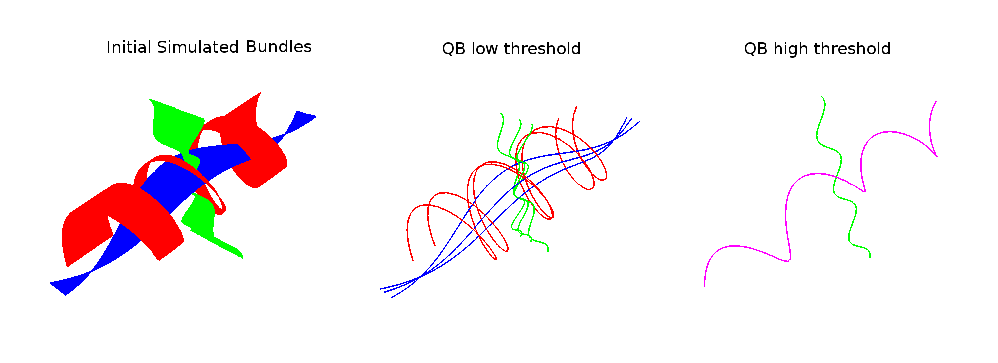
\includegraphics[width=160mm]{Figures/Fig_5_helix_phantom}
\par\end{centering}
\caption{Left: $3$ bundles of simulated trajectories; red, blue and
  green consisting of $150$ streamlines each. All $450$ streamlines are
  clustered together using QB. Middle and Right: centroid streamlines
  using thresholds $1$ and $8$ respectively.  At low threshold the
  underlying structure is reflected in a more detailed
  representation. At higher threshold, closer bundles merge
  together. Here the red and blue bundle have merged together in one
  cluster represented by the purple centroid
  streamline.\label{Flo:simulated_orbits}}
\end{figure*}

We can see similar effects with real streamlines, for instance those of
the fornix shown at the left panel of Fig.~\ref{Flo:QB_fornix} where we
can obtain different numbers of clusters at different thresholds. In
that way we can stress thinner or thicker sub-bundles contained inside
other bigger bundles.

%A full tractography containing $\num{250000}$ streamlines was clustered
%using QB with a distance threshold of $10$~mm
%(Fig.~\ref{Flo:QB_fornix}).  We produced a useful reduction of the
%initial tractography leaving only $763$ centroid streamlines. Bundles
%smaller than $10$ streamlines were then removed. Every streamline shown
%represents an entire cluster containing from $10$ to $\num{5000}$
%streamlines each.

\begin{figure*}[htp]
\centerline{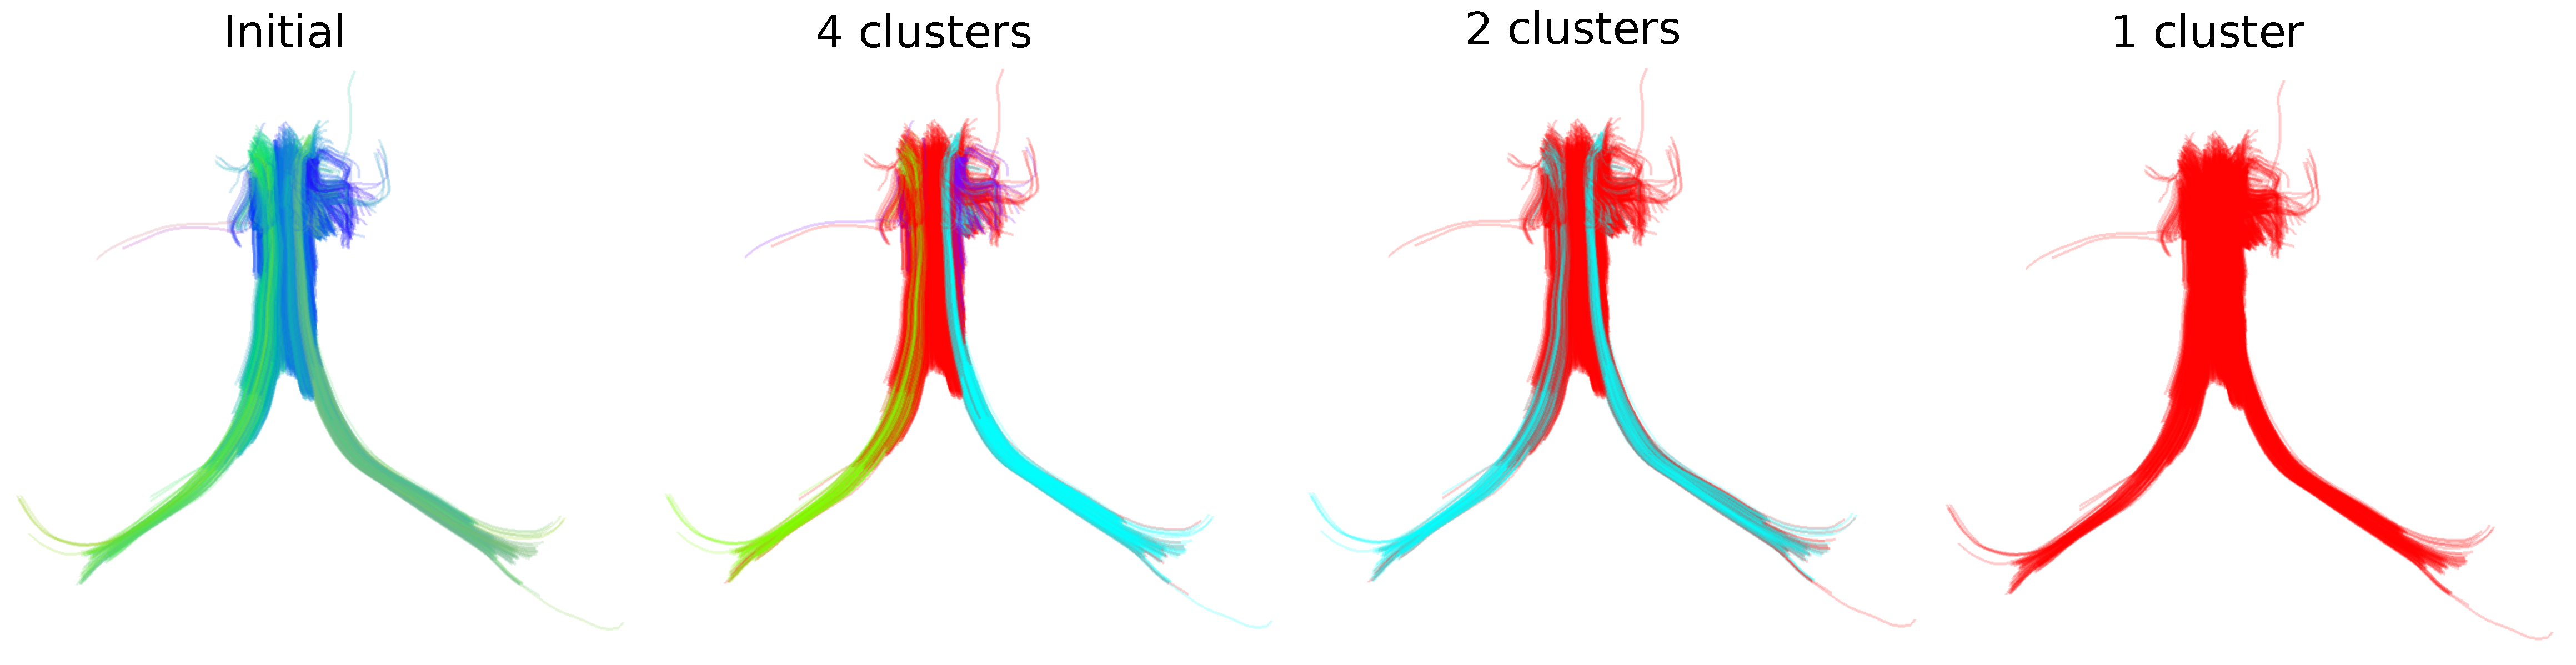
\includegraphics[width=160mm]{Figures/Fig_6_QB_fornix}}
\caption{QB clustering of the Fornix bundle. The original Fornix
  ($1076$ streamlines) is shown on the left panel using a standard
  orientation colormap. We observe that the Fornix consists of two long
  distant legs (left and right Fimbria) and a thicker upper part (Body
  of Fornix). We show here how QB will be able to distinguish the parts
  of the Fornix at different resolutions. With is a $15$~mm threshold QB
  generates 4 clusters shown on the second panel with distinct
  colors. Here the left and right Fimbria are clearly distinguished from
  the Body. A last cluster (with blue) exposes a shorter part of the
  Body which is probably due to noise in the data. With a $18$~mm
  threshold only two clusters are created. Both Fibria are brought
  together as one cluster. A property useful for studies which want to
  use both Fimbria as one. With a $20$~mm threshold the entire Fornix is
  one cluster. A case useful for interactive applications because now
  the entire Fornix can be described by only one centroid streamline. In
  all cases the streamlines of the Fornix were downsampled to have $18$
  points.\label{Flo:QB_fornix}}
\end{figure*}

In order to quantify the dimensionality reduction it achieves we applied
QB clustering to the 10 human subject data sets (\ref{sub:QB-Data-sets}). The mean
data compression (ratio of tractography size to number of QB clusters)
was $34.4:1$ with a $10$~mm threshold and $230.4:1$ with a $20$~mm
threshold.

%The centroid streamlines can be thought as fast access points to explore
%the entire data set (see Fig.~\ref{Flo:QB_fornix}). With an appropriate
%visualization tool we can click on a streamline and obtain the entire
%cluster/bundle that it represents. Visualizing an entire data set of
%this size is impossible on standard graphic cards and most visualization
%tools. For example Trackvis (trackvis.org) or DSI Studio
%(dsi-studio.labsolver.org) can only show a small random sample of the
%full tractography in real time. In addition we have developed fast and
%efficient ways of identifying broken or wandering streamlines by using
%the rapid data compression of QB to identify short or erratic centroid
%streamlines.

% \subsection{Medoid streamlines\label{sub:medoids}}

% The centroid streamlines created by QB have very nice properties as they
% represent an average streamline which can stand as the most
% characteristic feature of the cluster that they belong to. However, now
% that we have segmented our tractography into small bundles, we can
% calculate many more potentially important descriptors for the
% cluster. One of the most useful approaches is the calculation of
% medoids.

% Here the idea is to identify an actual streamline belonging to the
% tractography which corresponds in some way to the centroid streamline. In
% other words to find an medoid (medoid) streamline. Centroid streamlines
% do not necessarily coincide with real streamlines as they are just the
% outcome of large amalgamations. There are many strategies for how to
% select good medoids for the bundles. A very fast procedure that we use
% in our work is to find which real streamline from the cluster $c$ is
% closest (by MDF distance) to the centroid streamline $\mathbf{v}$. We
% will call this medoid streamline $\mathbf{e}_{1}$,
% i.e.~$\mathbf{e}_{1}={\displaystyle \argmin_{\mathbf{s} \in
%     c}}\textrm{\,\ MDF}(\mathbf{v},\mathbf{s})$.  The computational
% complexity of finding $\mathbf{e}_{1}$ is still linear in cluster size,
% and that will be very useful if we have created clusterings with
% clusters containing more than \textasciitilde5000 streamlines (depending
% on system memory).

% A different medoid can be defined as the most typical streamline among
% all streamlines in the bundle, which we denote by
% $\mathbf{e}_{2}={\displaystyle \argmin_{\mathbf{s} \in
%     c}}\,{\displaystyle \sum_{s'\in
%     c}}\mathrm{MDF}(\mathbf{s'},\mathbf{s})$, or if we want to work with
% streamlines with possibly different numbers of points we could instead
% use $\mathbf{e}_{3}={\displaystyle \argmin_{\mathbf{s} \in
%     c}}\,{\displaystyle \sum_{\mathbf{s'}\in
%     c}}\mathrm{MAM}(\mathbf{s'},\mathbf{s})$.  Here $\mathrm{MAM}$ can
% be any one of the Hausdorff MAM distance functions.  Identification of
% medoid streamlines of type $\mathbf{e}_{2}$ and $\mathbf{e}_{3}$ will
% be efficient only for small bundles of less than $5000$ streamlines
% because we need to calculate all pairwise distances in the bundle. We
% show below many applications of the medoids.

% In summary, a centroid (centroid) streamline is the average of all
% streamlines in the cluster. We call it centroid because it does not
% really exist in the real data set, and to distinguish it from medoid
% (medoid) streamlines which are again descriptors of the cluster but are
% represented by real streamlines.

\subsection{Comparison of clusterings\label{sub:Tightness-comparisons-1}}

We have found rather few systematic ways available in the literature to
compare different clustering results for tractographies directly, beyond
that of \citet{moberts2005evaluation} who quantified the agreement
between a clustering and a `gold standard' tractography labelled by
their team.  We have used a more symmetrical measure of agreement
between two clusterings that do not require a prior labelled data set.
It is called Optimised Matched Agreement (OMA). As with the Adjusted
Rand Index \citep{moberts2005evaluation}, OMA requires the calculation
of the $M \times N$ cross-classification matrix $X=(x_{ij})$ which
counts the number of streamlines in the intersection of all pairs of
clusters, one from each of the two clusterings.  Here
$\mathcal{A}=\{A_i:i=1\dots M\}$ and $\mathcal{B}=\{B_j:j=1\ldots N\}$
are the two clusterings, and $x_{ij}=|A_i \cap B_j|$. As there is no
\emph{a priori} correspondence or \emph{matching} between the
clusters in $\mathcal{A}$ and those in $\mathcal{B}$, and vice versa, we
need to find one empirically. If $j=\pi(i)$ is such a matching then the
matched agreement is $\mathrm{MA}(\pi) = \sum_{i=1}^M x_{i,\pi(i)}$. A
matching $\pi$ that yields OMA by maximising $\mathrm{MA}(\pi)$ can be
found using the Hungarian Algorithm~\citep{Kuhn1955}. The interpretation
of the OMA statistic is analogous to that of the well-known Kappa
measure of inter-rater agreement~\citep{altman1995}, with the range 61\%
to 80\% corresponding to a `good' strength of agreement.

As well as the computational overheads in calculating the
cross-classification matrix, a further fundamental disadvantage of these
methods is that they do not work with clusterings of different
tractographies.

Being able to compare results of clusterings is crucial for creating
stable brain imaging procedures, and therefore it is necessary to
develop a way to compare different tractography clusterings or different
sets of streamlines from the same subject or different subjects.

Although we recognise that these are difficult problems, we propose the
following approach with three novel comparison functions which we call
\emph{coverage}, \emph{sparsity} and \emph{bundle adjacency} (BA).

If $S$ and $T$ are sets of streamlines, and $\theta>0$ is selected as a
threshold, we say that $s \in S$ has a $\theta$-neighbour in $T$ if
$\min_{t\in T}[\mathrm{MDF}(s,t)<\theta]$; we define the coverage of $S$
by $T$ as the fraction of streamlines in $S$ that have a
$\theta$-neighbour in $T$: $|\{s \in S
\,\mathrm{has~a}~\theta\mathrm{-neighbour~in}~T\}|/|S|$; and we define
the sparsity of $T$ in $S$ as the average number of $\theta$-neighbours
in $T$ for streamlines in $S$. BA is a symmetric measure of the
similarity of the two sets of streamlines $S$ and $T$. BA is the average
of the $\theta$-coverages of $T$ by $S$ and of $S$ by $T$:
$\mathrm{BA}(S,T) = (\mathrm{coverage}(S,T) +
\mathrm{coverage}(T,S))/2$.

If $S$ is a good approximation to $T$ then $S$ will have high coverage
of $T$; if $S$ has low redundancy as an approximation to $T$ then the
sparsity of $S$ in $T$ will be low; and if $S$ and $T$ are globally
similar then BA will be high.

% Let us assume that we
% have gathered the centroid streamlines from clustering $A$ in
% $E_{A}=[\mathbf{e}_{1},...,\mathbf{e}_{M_{A}}]$ and from clustering $B$
% in $E_{B}=[\mathbf{e}_{1}^{'},...,\mathbf{e}_{M_{B}}^{'}]$ where $M_A$ ,
% $M_B$ denote the number of centroid streamlines of the two
% clusterings. $M_{A}$ does not need to be equal to $M_{B}$. Next we
% calculate all pairwise MDF distances between the two sets and store them
% in rectangular matrix $D_{AB}$. The mimima of the rows of $D_{AB}$
% provide the distance to the nearest streamline in $B$ of each streamline
% in $A$ ($m_{A\rightarrow B}$) and similarly the minima of the columns of
% $D_{AB}$ the distance to the nearest streamline in $A$ of each
% streamline in $B$ ($m_{B\rightarrow A}$). From these correspondences we
% only keep those distances that are smaller than a tight threshold
% $\theta$. Then we define BA to be

% \begin{equation}
% BA=\frac{1}{2}\left(\frac{|m_{A\rightarrow B}\leq \theta |}{M_{A}}+\frac{|m_{B\rightarrow A}\leq \theta |}{M_{B}}\right)\label{eq:TC}
% \end{equation}

% \noindent where $|m_{A\rightarrow B}\leq \theta |$ denotes the number of
% centroids from A which had a neighbour in B that is closer than $\theta$
% and similarly for $|m_{B\rightarrow A}\leq \theta |$.  In other words,
% $BA$ is mean of the fraction of row minima of $D_{AB}$ that are less
% than $\theta$ and the fraction of column minima less than $\theta$.
% $BA=0$ when every centroid from the one set is further than $\theta$ to
% all centroids in the other set. $BA=1$ when all centroids from one set have
% a close neighbour in the other set. This comparison function is very
% useful especially when comparing tractographies from different subjects
% because it does not require $M_{A}=M_{B}$.

% \subsection{Merging two sets of bundles\label{sub:merging}}

% \textbf{Do we keep this in?}

% We can merge bundles using medoid streamlines or centroid
% streamlines. We first set a distance threshold $\theta$ usually the same
% as the one we used for the QBs in the previous step. Assume now that we
% have gathered the centroid streamlines from clustering A in
% $V_{A}=[\mathbf{v}_{1},...,\mathbf{v}_{M_{A}}]$ and from clustering $B$
% in $V_{B}=[\mathbf{v}_{1}^{'},...,\mathbf{v}_{M_{B}}^{'}]$ where $M_A$
% and $M_B$ denote the number of centroid streamlines of each clustering.
% $M_{A}$ can be different from $M_{B}$. (1) For every
% $\mathbf{v}_{i}^{'}$ in $V_{B}$ we find the closest $\mathbf{v}_{j}$ in
% $V_{A}$ and store the distance between these two streamlines. Therefore
% we now have a set of minimum distances from $V_{B}$ to $V_{A}$. The size
% of this set is equal to $M_{B}|$. (2) We merge those clusters from B
% whose centroid streamlines have minimum distances (e.g. MDF) smaller than
% $\theta$ into the corresponding clusters of A, and if a centroid
% streamline in $V_{B}$ has no sub-threshold neighbour in $V_{A}$ then its
% cluster becomes a new cluster in the final clustering. In that way
% clusters from the two sets ho have very similar features will merge
% together, and, if not, new clusters will be created, and we will not
% have any loss of information from the two sets of clusters.

\subsection{\label{sub:QB-Data-sets}Data sets}

We applied QuickBundles to a variety of data sets: simulations, $10$
human tractographies collected and processed by ourselves, and one
tractography with segmented bundles which was available online.

\textbf{Simulated trajectories.} We generated $3$ different bundles of
parametric paths sampled at $200$ points. The streamlines were made from
different combinations of sinusoidal and helicoidal functions.  Each
bundle contained 150 streamlines.  For the red bundle in
Fig.~\ref{Flo:simulated_orbits} a pencil of helical streamlines all
starting at the same point on a cylinder was generated by linearly
varying the pitch of the helices; the green bundle was made up from a
divergent pencil of rays on a sinusoidally corrugated sheet; the blue
bundle is similarly made from a divergent rays on a sinsusoidally
corrugated sheet, with the rays undergoing sinusoidal modulated lateral
bending over a range of amplitudes.

\textbf{Human subjects.} We collected data from $10$ healthy subjects at
the Medical Research Council's Cognition and Brain Sciences Unit with a 3~Tesla
scanner (TIM Trio, Siemens), using a Siemens advanced diffusion
work-in-progress sequence, and STEAM \citep{merboldt1992diffusion,MAB04}
as the diffusion preparation method. The field of view was
$240\times240\,\textrm{mm}^{2}$, matrix size $96\times96$, and slice
thickness $2.5\,\textrm{mm}$ (no gap).  $55$ slices were acquired to
achieve full brain coverage, and the voxel resolution was
$2.5\times2.5\times2.5\,\textrm{mm}^{3}$. A $102$-point half grid
acquisition \citep{Yeh2010} with a maximum $b$-value of $4000\,
\textrm{s/mm}^{2}$ was used.  The total acquisition time was $14'\,21''$
with TR=$8200\,\textrm{ms}$ and TE=$69\,\textrm{ms}$. The experiment was
approved by the Cambridge Psychology Research Ethics Committee (CPREC).

For the reconstruction of the $10$ human data sets we used Generalized
Q-Sampling \citep{Yeh2010} with diffusion sampling length $1.2$ and for
the tractography propagation we used EuDX (Euler integration with
trilinear interpolation, \citet{Garyfallidis_thesis}), angular threshold
\ang{60}, total weighting $0.5$, propagation step size $0.5$ and
quantitative anisotropy stopping threshold $0.0239$ (see
Fig.~\ref{Flo:arcuate_close}).

\textbf{PBC human subjects}. We also used labelled data sets by
experts(see Fig.~\ref{Flo:cst_pbc} and \ref{Flo:QB_fornix}), from the
freely available tractography database used in the Pittsburgh Brain
Competition Fall $2009$, ICDM (pbc.lrdc.pitt.edu).

\end{methods}

\section{Results}

In this section we justify our claims about the speed and linear
complexity of QB (\ref{sub:Complexity}). Next we demonstrate the
robustness of QB as a method for clustering tractographies
(\ref{sub:Comparisons}). In \ref{sub:group_comp} we show a new way to
find similarities across different tractographies and
in \ref{sub:short_tracks} we discuss about some potential limitations
of our methods and possible workarounds.

% XXX WHERE THIS SHOULD GO?
% In \ref{QB_Representation} we illustrate the high level of clarity and
% simplification that the QB representation can bring to a tractography,
% and how adjustment of the distance threshold $\theta$ can be used to
% merge or split clusters.

% In \ref{sub:Atlases-made-easy} we show how the
% QB representations for a group of subjects can be mapped into a common
% space and then reclustered to generate a multi-subject atlas of white
% matter tractographies. We show moreover how the resulting atlas can be
% used to access clusters in the individual tractographies that have a
% good correspondence bewteen subjects. Both the speed of performance and
% the data reduction provided by QB make this innovation a practical
% research tool. 
%Tractography clustering algorithms have not to date been able to work on
%full tractography data sets. 
% We show in \ref{sub:QB_as_input} how using
% the QB representation of the tractography as input to higher complexity
% clustering methods brings full tractographies within their effective
% range.
% We indicate
% (\ref{sub:exemplars_vs_ROIs}) medoids streamlines from the QB
% representation can improve on interaction with tractographies and can be
% used for the direct registration of tractographies
%(\ref{sub:direct_registration}).  
% \noindent
%Finally, quality control of tractographies is an important issue and we
%show how QB can be used as a fast tool to identify clusters containing
%long or short streamlines (\ref{sub:short_tracks}).

\subsection{Complexity and timings\label{sub:Complexity}}

To apply QB to a data set we need to specify three key parameters: $K$,
the fixed number of downsampled points per streamline; $\theta$ the
distance threshold, which controls the heterogeneity of clusters; and
$N$ the size of the subset of the tractography on which the clustering
will be performed. When $\theta$ is higher, fewer more heterogeneous
clusters are assembled, and conversely when $\theta$ is low, more
clusters of greater homogeneity are created.

The complexity of QB is in the best case linear time $\mathcal{O}(N)$
with the number of streamlines $N$ and worst case $\mathcal{O}(N^{2})$
when every cluster contains only one streamline. The average case is
$\mathcal{O}(MN)$ where $M$ is the number of clusters however because
$M$ is usually much smaller than $N$ ($M\ll N$) we can neglect $M$ and
denote it only as $\mathcal{O}(N)$ as it is common in complexity
theory. We created the following experiment to investigate this claim
and we found empirically that the average case is actually
$\mathcal{O}(N)$ for tractographies (see Fig.\ref{Flo:Speed1}).  In this
experiment we timed the duration of QB clustering of tractographies
containing from \num{50000} to \num{500000} streamlines in steps of
\num{50000}, with $12$ points per streamline and different QB thresholds
($20,25,30$~mm). These results were obtained using a single thread
Intel(R) CPU E5420 at 2.50GHz on a standard notebook. The results for a
single subject can be seen in Fig.~\ref{Flo:Speed1}. The same pattern
was observed for the remaining $9$ subjects. This experiment concludes
that QB is suitable for fast and linear time clustering of
tractographies.

\begin{figure}
\noindent \begin{centering}
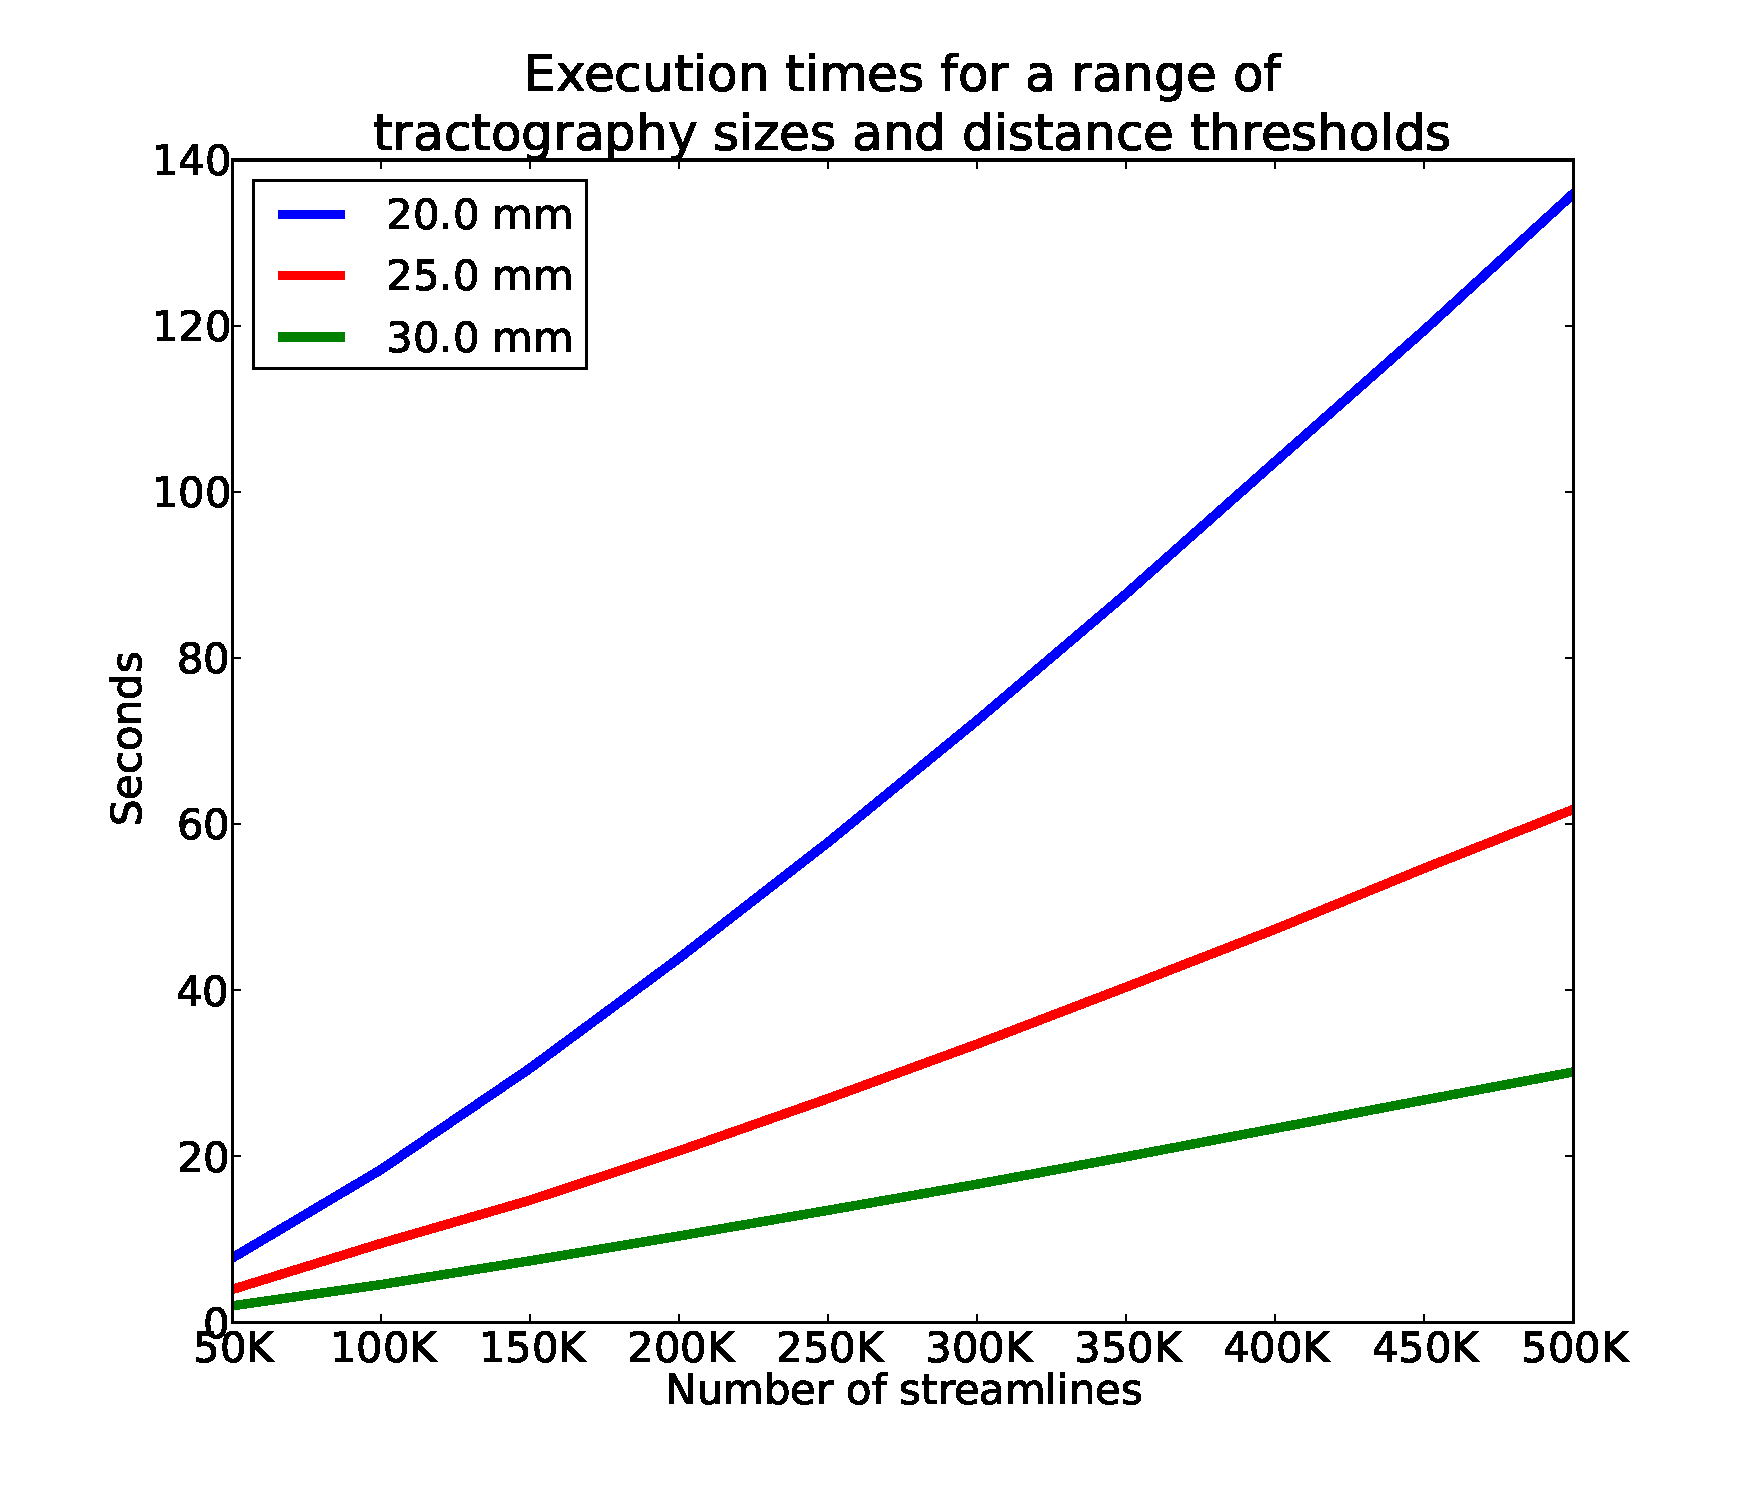
\includegraphics[scale=0.3]{Figures/Fig_3_timings}
\par\end{centering}
\caption{Time comparisons of QB using different distance thresholds and
  different number of streamlines. Time increases linearly as the number
  of streamlines increases. \label{Flo:Speed1}}
\end{figure}

As a further test we compared QB with $12$ point streamlines and a
distance threshold of $10$~mm with some timings reported from other
state of the art methods found in the literature. Unfortunately timings
have be rather rarely reported up till today -- possibly because as most
algorithms were very slow on full data sets. With $\num{1000}$
streamlines \citet{wang2010tractography}'s algorithm took $30$ whereas
QB took $0.07$.  $\num{14400}$ seconds were required for the method of
\citet{wang2010tractography} to cluster $\num{60000}$ streamlines; QB
took $14.7$.  In a third study a substantial tractography of size
$\num{400000}$ was clustered by \citet{Visser2010} in $\num{75000}$; QB
completed this task in $160.1$. The speed-up factors in these three
comparisons were $429$, $980$ and $468$ respectively.  Though this
experiment was performed using a single CPU core we see the valuable
speedup that QB achieves, holding out the prospect of real-time (less
than 1~second) clustering on data sets of up to \num{20000} streamlines.
% (see Table~\ref{Flo:timings}).

% \begin{table}
% \scriptsize\addtolength{\tabcolsep}{-5pt}
% \caption{Performance timings for QB compared with some timings
%   reported in the literature.\label{Flo:timings}}
% \begin{centering}
% \begin{tabular}{ccccc}
% \hline 
% %\hline
% Number of streamlines ($N$) & Algorithms & Timings (secs) & QB (secs) & Speedup\tabularnewline
% \hline
% $1000$ & \citet{wang2010tractography} & $30$ & $0.07$ & $429$\tabularnewline
% $\num{60000}$ & \citet{wang2010tractography} & $\num{14400}$ & $14.7$ & $980$\tabularnewline
% $\num{400000}$ & \citet{Visser2010} & $\num{75000}$ & $160.1$ & $468$\tabularnewline
% \hline
% \end{tabular}
% \par\end{centering}
% \end{table}

\subsection{Stability of QB \label{sub:Comparisons}}

One of the disadvantages of most clustering algorithms is that they give
different results with different initial conditions; for example this is
recognised with k-means, expectation-maximization
\citep{dempster1977maximum} and k-centers \citep{gonzalez1985clustering}
where it is common practice to try a number of different random initial
configurations. The same holds for QB so if there are not distinct
clusters such that the distance between any pair of clusters is
supra-threshold and the diameter of all clusters is sub-threshold, then
with different permutations of the same tractography we will typically
see similar number of clusters but different underlying clusters. We
will examine the robustness of QB in this respect.

As a first step we recorded the numbers of QB clusters in $20$ different
random orderings of the tractographies of $10$ human subjects acquired
as described in section \ref{sub:QB-Data-sets}. We first removed short
streamlines shorter than $40$~mm and downsampled the streamlines at $12$
points. Then we applied QB with threshold at $10$~mm. The mean number of
clusters was $2645.9$ (min $1937.6$; max $3857.8$; s.d.~$653.8$). There
is therefore a considerable between-subject variation in this metric. By
contrast the within-subject variability of the number of clusters across
random orderings is rather small, with mean standard deviation $12.7$
(min $7.3$; max $17.4$). This suggests a good level of consistency in
the data reduction achieved by QB.

Next we investigated how consistent QB clusterings are when data sets
are re-ordered. Twelve different random ordering were generated for each
of $10$ tractographies and the corresping QB clusterings were computed
with MDF threshold $10$~mm. For each subject the $66$ pairings of QB
clusterings were compared using the optimised matched agreements index
and then averaged. Across subjects the mean OMA
(\ref{sub:Tightness-comparisons-1}) was 74.1\% ($\pm 0.39$\%) which can
be interpreted as a good level of agreement~\citep{altman1995}.

As well as checking that QB created sets of centroids with good coverage
and sparsity statistics, we went on to show that the performance of QB
generalises to sets of streamlines different from the training set, and
is superior to a random sample of streamlines. We split each of the 10
tractographies randomly into two halves $T_1$ (training set) and $T_2$
(test set). The QB clustering at distance threshold $10$~mm was derived
for $T_1$. Denote by $C_1$ and $c_1$ the set of centroids and the number
of them. Let $R_1$ be a random subset of $T_1$ of size $c_1$. Using the
measures described in section~\ref{sub:Tightness-comparisons-1} we found
that with closeness threshold $10$~mm the mean coverage (s.d.) of $T_1$
by $C_1$ was $99.96$\% ($\pm 0.007$\%), of $T_2$ by $C_1$ was $99.31$\%
($\pm 0.08$\%) and of $T_2$ by $R_1$ was $90.49$\% ($\pm 0.41$\%). The mean
sparsity (s.d.) at this threshold of $C_1$ in $T_1$ was $2.44$ ($\pm
0.08$), of $C_1$ in $T_2$ was $2.44$ ($\pm 0.08$), and of $R_1$ in $T_2$
was $5.57$ ($\pm 0.50$).

The same analyses were performed with QB clusterings for distance
threshold $20$mm and with distance threshold $20$mm. (Note that though
we have selected the same values here for the two threshold they do not
have to be the same.) We found that with distance threshold $10$mm the
mean coverage (s.d.) of $T_1$ by $C_1$ was $99.99$\% ($\pm 0.004$\%), of
$T_2$ by $C_1$ was $99.91$\% ($\pm 0.02$\%) and of $T_2$ by $R_1$ was
$95.86$\% ($\pm 0.62$\%). The mean sparsity (s.d.) at this threshold
of $C_1$ in $T_1$ was $3.54$ ($\pm 0.18$), of $C_1$ in $T_2$ was $3.54$
($\pm 0.18$), and of $R_1$ in $T_2$ was $6.53$ ($\pm 0.93$).

We conclude from these analyses that QB has good coverage and sparsity
both the training set and the test set of streamlines, while an
equivalent random selection of streamlines has worse coverage and
sparsity. Moreover the performance of QB is better with the lower
closeness threshold. The poor performance of random subsets is to be
expected as they will oversample in dense parts of the tractography
space, and undersample in sparser regions.

% \subsection{Tractographic atlases and landmarks\label{sub:Atlases-made-easy}}

% We have used QB to construct a robust tractographic atlas in MNI space
% with data from 10 subjects. First we used the FSL toolbox using steps
% similar to those in~\citet{Smith2006NeuroImage} to register each
% subject's FA volume with the standard FSL template (\texttt{FMRIB58}) in
% MNI space. Next we applied the resulting non-linear transformations to
% the tractographies. This required technical solutions which are detailed
% in the DIPY software package.

% Having all tractographies in MNI space is especially useful because we
% can now compare them against available templates or against each other
% and calculate different statistics. However this is not where we stop;
% we proceed to generate a tractographic atlas using QB clusterings.

% \textbf{Tractographic Atlases} For each subjects, (a) load the warped
% tractography, (b) downsample the streamlines to have only $12$ points, (c) calculate
% and store QB clustering with a $10$~mm threshold, (d) merge all
% clusterings again with a $10$~mm threshold as explained in
% section~\ref{sub:merging}. When creating an atlas by merging
% many different subjects the most important issue is what one removes
% from the atlas as outliers.  QB here provides a possible solution for
% this problem. From the distribution of cluster sizes we find that $20\%$
% of the largest clusters had more than $90\%$ of all streamlines. This shows
% that there is much agreement between the biggest bundles of different
% subjects.  We will use this property to create a solid atlas in which we
% keep the biggest bundles (landmarks) and remove small bundles
% (outliers).

% This atlas has been constructed without considering whether there are
% inter-subject differences in white matter organisation. Outliers might
% represent genuine differences in anatomy and the corresponding atlas
% clusters can be explored to see how many subjects they relate to. With a
% larger database QB can thus be used to create a probabilistic
% tractography atlas with which to identify differences in morphology in
% an analogous manner to that achieved for the cingulate and parasingulate
% sulci by \citet{paus1996human}.

% \textbf{Finding and Using Landmarks} One can use this atlas or similar
% atlases created from more subjects in order to select specific
% structures and study these structures directly in different subjects
% without using any of the standard ROI based methods.

% A simple example is given in Fig.~\ref{Flo:CloseToSelected}. In the
% first row we see a tractographic atlas joined by merging the QB
% clusterings of $10$ healthy subjects as described in the previous
% section. Then from these clusters represented by their centroid streamlines we
% keep only $196$ biggest clusters i.e. those which contain the highest
% number of streamlines, so that we are sure that there is enough agreement
% from the different tractographies. From these we pick by way of an
% example $19$ centroid streamlines (see Tab.~\ref{Flo:structures} which
% correspond to well known bundle structures in the literature:

% \begin{table}
% \small\addtolength{\tabcolsep}{-5pt}
% \caption{The 17 fiber bundles chosen for the analysis in Fig.~\ref{Flo:CloseToSelected}.\label{Flo:structures}}
% \begin{centering}
% \begin{tabular}{lll}
% \hline 
% %\hline
% Abbreviation & Structure \tabularnewline
% \hline
% GCC   & genu of corpus callosum \tabularnewline
% BCC   & body of corpus callosum \tabularnewline 
% SCC   & splenium \tabularnewline
% CP    & pons cerebellar peduncle \tabularnewline
% ARC-L & left arcuate fasciculus \tabularnewline
% ARC-R & right arcuate fasciculus \tabularnewline
% IFO-L & left inferior occipitofrontal fasciculus \tabularnewline
% IFO-R & right inferior occipitofrontal fasciculus \tabularnewline
% FX-R  & right fornix \tabularnewline
% FX-L  & left fornix  \tabularnewline
% OR    & optic radiation  \tabularnewline
% CGL-L & left cingulum  \tabularnewline
% CGL-R & right cingulum  \tabularnewline
% CST-L & left corticospinal tract  \tabularnewline
% CST-R & right corticospinal tract \tabularnewline
% UNC-L & left uncinate \tabularnewline
% UNC-R & right uncinate \tabularnewline
% \hline
% \end{tabular}
% \par\end{centering}
% \end{table}

% These $19$ streamlines are coloured randomly. Then on the second row we show,
% for the first $6$ of these selected centroid streamlines, the streamlines
% closer than $20$~mm from $3$ arbitrarily selected subjects. Similarly,
% on the third row the streamlines closer than $15$~mm to the next $7$ selected
% streamlines. Finally on the last row we bring the streamlines from the same $3$
% subjects which are closer than $18$~mm.  The colours used for the
% selected streamlines are automatically assigned from the colours assigned to
% the streamlines picked from the atlas. We can see that there is a significant
% reliability and continuity both within and between subjects even though
% we have only selected a very small number of centroid
% streamlines. Using a similar procedure we could create a list of bundles of
% every subject and then compare the subjects at the level of bundles.

% %
% \begin{figure}
% \begin{centering}
% 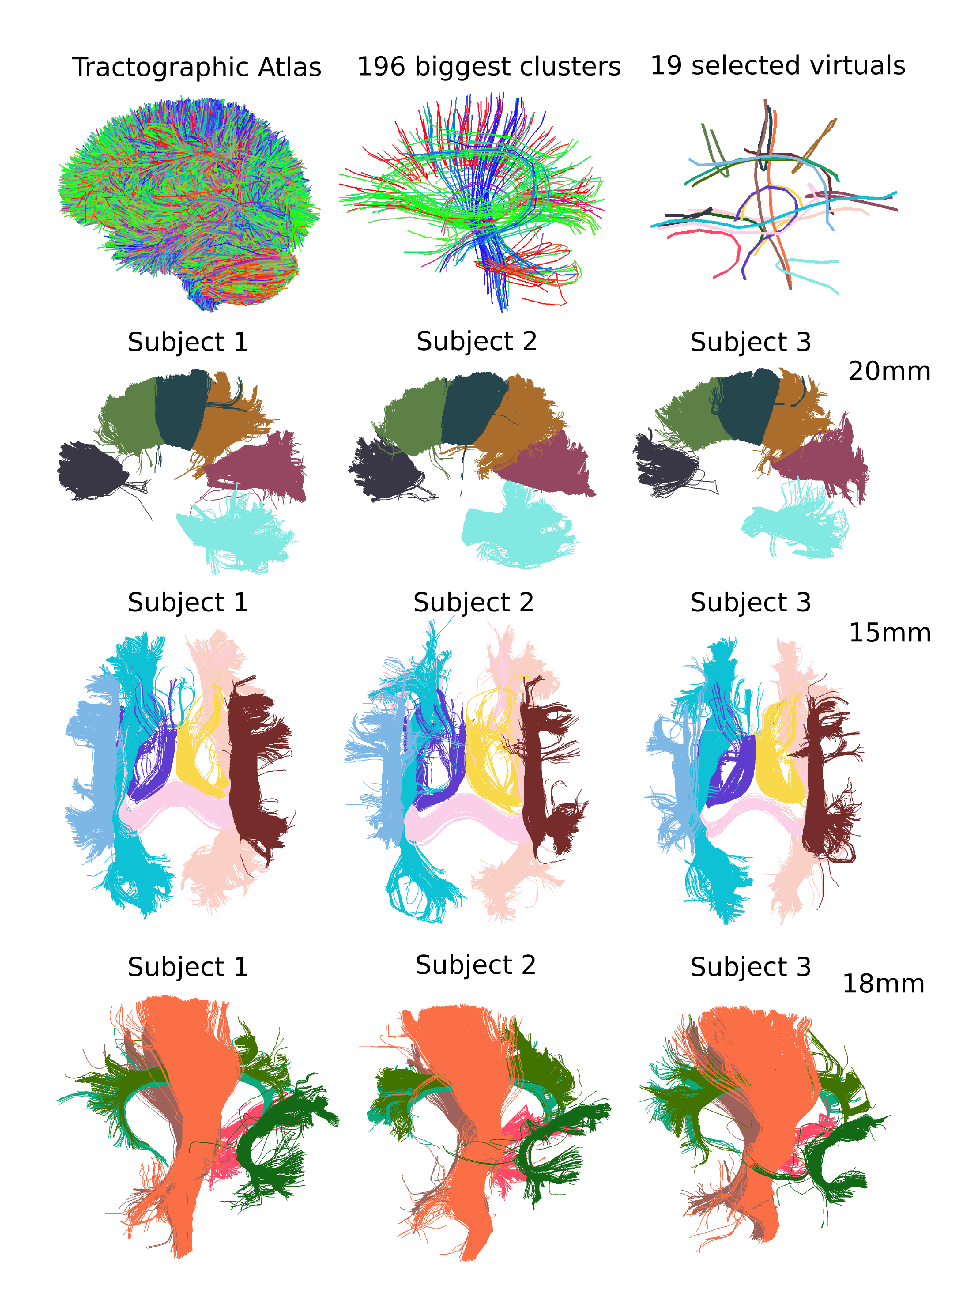
\includegraphics[scale=0.5]{Figures/Fig_7_close_distance}
% \par\end{centering}
% \caption{A novel way to do comparisons between subjects. Correspondence
%   between different subjects (last $3$ rows) and a few landmarks picked
%   from the tractographic atlas generated by merging QB clusterings of
%   $10$ subjects (top row). The fact that we can see this amount of
%   agreement and continuity on the last $3$ rows from so few centroid
%   streamlines provides a new robust way to statistical comparison between
%   tractographic data sets. (Rows 3 and 4 are from different viewpoints
%   from that in rows 1 and 2.) \label{Flo:CloseToSelected}}
% \end{figure}

% \subsection{QB as input to higher complexity methods\label{sub:QB_as_input}}

% We found that QB is of great value as an adjunct to many less efficient
% algorithms e.g.~hierarchical clustering, affinity propagation, nearest
% neighbours, spectral clustering and other unsupervised and supervised
% machine learning methods. We present here one example with QB as input
% to affinity propagation and one with QB as input to hierarchical
% clustering.

% Most clustering algorithms need to calculate all pairwise distances
% between streamlines; that means that for a medium sized tractography of
% \num{250000} streamlines we would need $232$ GBytes of RAM with single
% floating point precision. Something which is not and will not be
% available soon in personal computers. In those cases some people might
% hope that sparse matrices could provide a nice approximation; however
% dense tractographies produce very dense distance matrices. The
% straightforward solution to this problem is to use QB in order to first
% segment in small clusters and then use the representative streamlines
% (i.e. medoid or centroid streamlines) of these clusters with other
% higher complexity operations and merge the clusters together in bigger
% clusters.

% The required steps are: (1) cluster each tractography using QB as
% explained in section~\ref{sub:Atlases-made-easy}); (2) gather up the
% centroid streamlines; (3) calculate MDF distances between the centroid
% streamlines; (4) use any other clustering method to segment this much
% smaller distance matrix $D$.

% In the left panel of Fig.~\ref{Flo:LSC+HC+AP} we show a result where we
% used hierarchical clustering with single linkage for step (4) with a
% threshold of $20$~mm using the Python software package
% $\texttt{hcluster}$~\cite{eads-hcluster-software}. A known drawback of
% single linkage is the so-called chaining phenomenon: clusters may be
% brought together due to single elements being close to each other, even
% though many of the elements in each cluster may be very distant to each
% other. Chaining is usually considered as a disadvantage because it is
% too driven by local neighbours. Nevertheless, we can take advantage of
% this property to cluster the entire corpus callosum (CC) together (shown
% in dark red in left top of Fig.~\ref{Flo:LSC+HC+AP}) creating a fully
% automatic CC detection system.  Furthermore, we can use different
% cutting thresholds on the underlying dendrogram to amalgamate together
% different structures (see e.g.~the cingulum bundles in the same panel).

% In the right panel of Fig.~\ref{Flo:LSC+HC+AP} we see an implementation
% of step (4) using the more recent algorithm, affinity propagation
% (AP)~\citep{dueck2009affinity}, which has been
% identified~\citep{malcolm2009filtered}) as being difficult or impossible
% to be used for group analysis or to cluster entire tractographies of
% many thousands of streamlines.

% Here we see in the bottom right panel of (see Fig.~\ref{Flo:LSC+HC+AP})
% how nicely AP, after the simplification provided by QB, has clustered
% arcuate, longitudinal occipitofrontal fasciculus and other structures
% known from the literature. The input of AP was the negative distance
% matrix $-D$, the preference weights were set to matrix
% $\mathtt{median}(-D)$ and the hierarchical clustering parameter was set
% to $20$~mm.  For affinity propagation we used the Python library
% \texttt{scikit-learn}.

% \begin{figure}
% \begin{centering}
% 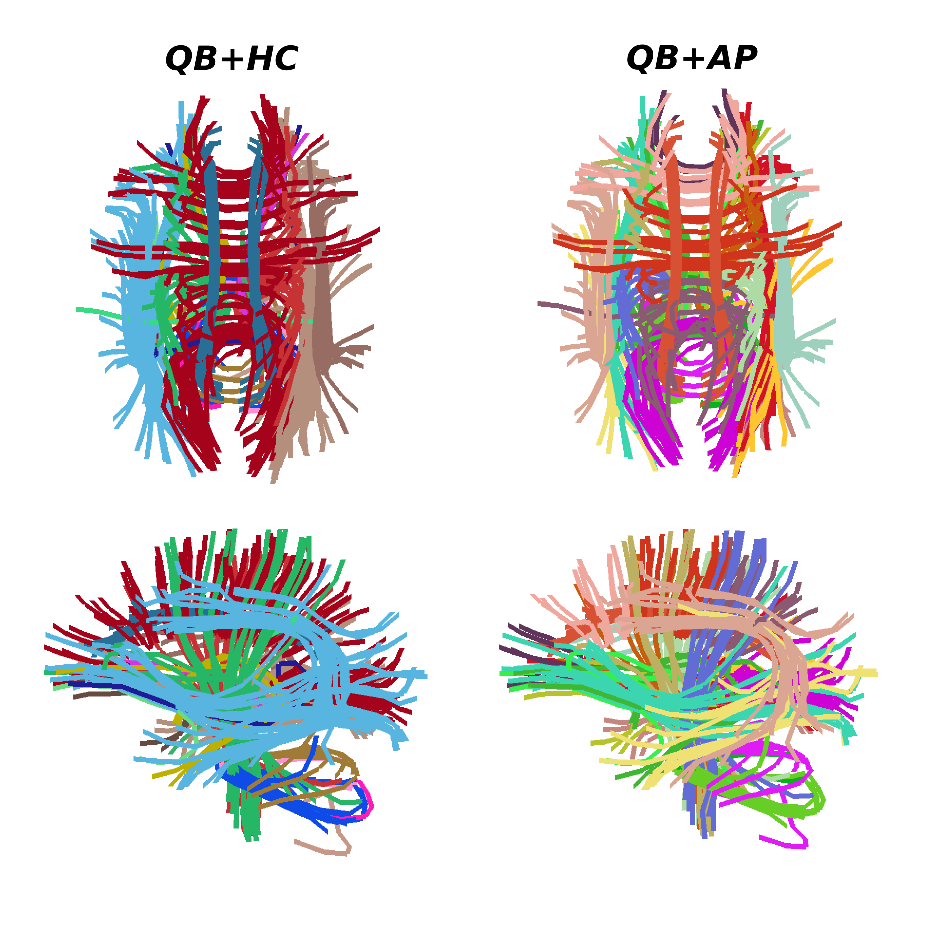
\includegraphics[scale=0.6]{Figures/Fig_8_QB_with_others}
% \par\end{centering}
% \caption{QB was used to cluster an entire set of $10$ tractographies
%   together (\num{2500000} streamlines). The resulting QB representation
%   was used as input to hierarchical clustering (HC) using single linkage
%   (left) and to affinity propagation (AP, right). Colours encode cluster
%   labels. HC results in 19 clusters, AP in 23. QB facilitates
%   significantly the operation of the other two algorithms which would
%   not be able to cluster the entire data sets on current computers. Note
%   the top left panel where QB+HC have managed to cluster the entire CC
%   in one bundle.\label{Flo:LSC+HC+AP}}
% \end{figure}

% While clustering methods of higher order complexity such as HC and AP
% have considerable theoretical appeal and have a deserved reputation for
% being able discover meaningful structure in data sets they are simply
% impracticable when more than a few thousand items are being
% clustered. Using QB to pre-process the tractography puts the whole data
% set, condensed to its centroid streamlines, within the feasible range of
% these higher order algorithms.

% \subsection{Medoids replace ROI masks\label{sub:exemplars_vs_ROIs}}

% Medical practitioners and neuroanatomists often argue that when they use
% multiple spherical or rectangular masks to select some bundles many
% streamlines are thrown away because they are small and the mask operations
% cannot get hold of them. Our method provides a solution to this problem
% as it can identify broken or smaller bundles inside other bigger bundles
% which are otherwise very difficult or even sometimes impossible to
% identify visually or with the use of masks. Our method attacks this
% problem and suggests a very efficient and robust solution which sets the
% limit for unsupervised clustering of tractographies and facilitates
% tractography exploration and interpretation. The point here is that one
% can now use medoid streamlines as access points into the full tractography
% and with a single click on that medoid streamline obtain the entire bundle.
% Therefore a super-bundle can be created just with with a few clicks
% based on a selection from medoid streamlines.

% In order to create this system we implemented a 3D
% visualization/interaction system for tractographies based on QB in
% Python and OpenGL. This code is available online at $\texttt{fos.me}$.


% \subsection{Direct Tractography Registration\label{sub:direct_registration}}

% Direct tractography registration is a recently described problem with
% only a small number of publications \citep{leemans2006multiscale,
%   mayer2008bundles, mayerdirect, mayer2011supervised,
%   durrleman2010registration, zvitia2008adaptive, Zvitia2010,
%   ZiyanMICCAI07}, and so far as we know there are no publicly available
% solutions. By direct registration we mean that no other information
% apart from the tractographies themselves is used to guide the
% registration. This is in contrast to
% section~\ref{sub:Atlases-made-easy}) where we used FA registration
% mappings applied to tractographies which is also most commonly used in
% the literature along with other Tensor based
% methods~\cite{goh2006algebraic}.

% We now describe our algorithm which is efficient and simple
% to use, completely automatic and provides an evidently robust direct
% rigid tractography registration algorithm available in seconds. This
% algorithm could be of great use when comparing healthy versus severely
% diseased brains e.g.~stroke or vegetative state patients when non-rigid
% registration is not recommended because of severe asymmetries in the
% diseased brains. The algorithm is based on the robustness of QB to find
% good representative descriptors.

% Let $T_{A}$, and $T_{B}$ the two tractographies to be aligned in native
% space. The required steps are: (1) all streamlines with length smaller than
% $100$~mm and longer than $300$~mm are removed from the data sets. (This
% will reduce the size of each tractography to about $1/4$ of its initial
% size i.e.~\textasciitilde \num{200000} streamlines. While all the subjects
% are adults, this filtering may have different effects depending on brain
% size. We have not investigated this question at present); (2) downsample
% both tractographies equidistantly to $12$ points; (3) run QB with
% distance threshold at $10$~mm for both tractographies; (4) collect all
% medoid streamlines from clusters containing more than $0.2\%$ of all
% streamlines; (5) assuming we have these now in $E_{A}$ and $E_{B}$, calculate
% all pairwise distances $D=\mathtt{MDF}(E_{A},E_{B})$ and save them in
% rectangular matrix $D$; (6) use the modified Powell's method
% \citep{fletcher1987practical} to minimize the symmetric distance
% function $\mathrm{SMD}=\sum_{i}\min_{j}D(i,j)+\sum_{j}\min_{i}D(i,j)$
% over rigid rotations of $E_{B}$ starting with zeroed initial conditions;
% (7) after each iteration of the optimization, $E_{B}$ is transformed by
% the resulting rigid rotation and $\mathrm{SMD}$ is recalculated. To
% ensure smooth rotations we use the Rodriguez rotation formula.

% In Fig.\ref{Flo:direct_registration} A we see the result of this
% algorithm applied to two tractographies represented by their
% medoid streamlines, depicted in orange and purple. We can see in the
% upper panel that the orange tractography is misaligned with respect to
% the purple one, and in the lower panel we see their improved alignment
% after applying our algorithm.

% \textbf{Metric}. SMD is proposed here for registration of trajectory
% data sets, but one could equally use mutual
% information~\citep{maes1997multimodality} or the correlation
% ratio~\citep{roche1998correlation} for registration of volumetric data
% sets. Nonetheless, the advantage of SMD is that it comes from robust
% landmarks generated by QB which bring together local and global
% components. Initially, it was not clear if we should use SMD or just the
% sum of all distances $\mathrm{SD}=\sum_{i,j}D(i,j)$. Therefore, we made
% a small experiment to validate the smoothness and convexity of these two
% cost functions. We plotted both functions under a single-axis
% translation or a single-angle rotation of the same tractography as show
% in Fig.~\ref{Flo:direct_registration} B and C. From, these two diagrams
% we can see that although for translations only the SD was entirely
% convex, with rotations the SD had stronger local minima which is not a
% good property for registration. Furthermore, the SMD had steeper
% gradients towards the global minimum which is a positive indicator for
% faster convergence.

% \textbf{Experiments}. The first large scale experiment took place using
% the same tractography of a single individual copied and transformed
% $1000$ times with range of all three angles from \ang{-45} to \ang{45}
% and range of all x,y,z translations from \numrange{-113}{113}~mm. Then
% we registered all transformed tractographies to the static one and
% calculated all pairwise MDF distances storing them in a square matrix
% $D$. We would expect that if the registration was correct then the sum
% of all diagonals elements of $D$ would be close to $0$. This was
% confirmed with both cost functions used SD and SMD getting close to zero
% $99.8\%$ of the time however SMD was always closer to perfect alignment
% than SD. Consequently we chose SMD as a better cost function for direct
% tractography registration.

% We used GQI-based tractographies from $10$ subjects, and registered all
% 45 possible pairs. Comparing different tractographies is not a trivial
% problem however we can use the bundle adjacency (BA) metric explained in
% section \ref{sub:Tightness-comparisons-1}.  We can report that the mean
% initial BA was $34.8\%\pm8.0\%$ and the mean final BA after applying our
% direct registration method was $48.1\%\pm6.1\%$. This was a
% statistically highly significant improvement
% ($t_{\text{\textrm{paired}}}(44)=11.2$, $p\leq10^{-13}$). These BA
% values are comparable to those reported in
% section~\ref{sub:Tightness-comparisons-1}. We are planning in the future
% to compare this registration method against other standard methods which
% are common in the literature.

% It should be noted that both BA and SMD are derived from the same
% distance matrix $D_{AB}$ between the two sets of centroid
% streamlines. However, using BA to assess a registration that has minimised
% SMD is less circular than might appear at first sight; the minimization
% of SMD depends on all the entries of $D$ as it is the mean of all those
% entries, while BA depends on the separate minimizations of the rows and
% columns of $D$.

% \begin{figure}
% \begin{centering}
% 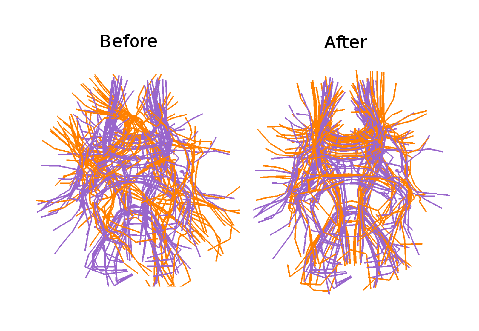
\includegraphics[scale=1.0]{Figures/Fig_9_QB_registration2_only_landscape}
% \par\end{centering}
% \caption{Tractographies from two different subjects
%   before (left) and after (right) QB-based direct registration.\label{Flo:direct_registration}}
% \end{figure}


\begin{figure*}[htp]
  \centerline{\includegraphics[width=180mm]{Figures/Fig_12_All_Brains.eps}}
  \caption{QuickBundles centroids of the biggest 100 clusters for 10
    subjects. Full tractographies are also presented using high
    transparency. All streamlines are visualized with the same standard
    orientation colormap. \label{Flo:BAs}}
\end{figure*}


\subsection{Group Comparisons \label{sub:group_comp}}

We warped $10$ tractographies each belonging to a different healthy
subsect (see section \ref{sub:QB-Data-sets}) in MNI space and applied
QuickBundles on each tractography independently using distance threshold
$10$~mm and downsampling of $18$ points. For every subject we
only considered the biggest $100$ QB clusters i.e. the clusters which
contained the highest number of streamlines. The purpose of this
experiment was to identify a global similarity measure between the
streamlines of the different subjects.

In Fig.~\ref{Flo:BAs} we present both the complete tractographies and
the centroid tracks which correspond to the $100$ biggest
clusters. Because the complete tractographies are very large containing
hundreds of thousands of tracks (mean$=\num{171002.5}\pm\num{23879.9}$)
we visualize them using low opacity so that at least an overall
projection of the streamlines can be observed. The purpose of this is to
show empirically the variability of the streamlines across subjects. At
the contrary, the centroids of the $100$ biggest clusters for the $10$
subjects are easily observed with full opacity in
Fig.~\ref{Flo:BAs}. The mean number of streamlines in the $100$ biggest
clusters was $\num{4818.6}$ ($\pm \num{794.4}$). These clusters covered
on average $16.18\%$ ($\pm\num{1.4}\%$) of the total number of
streamlines. The average length of the centroids of the clusters was
$73.6$~mm ($\pm\num{43.9}$~mm). We will use these centroids as a method
to study the variability between the streamlines across different
subjects.

\begin{figure}
\centerline{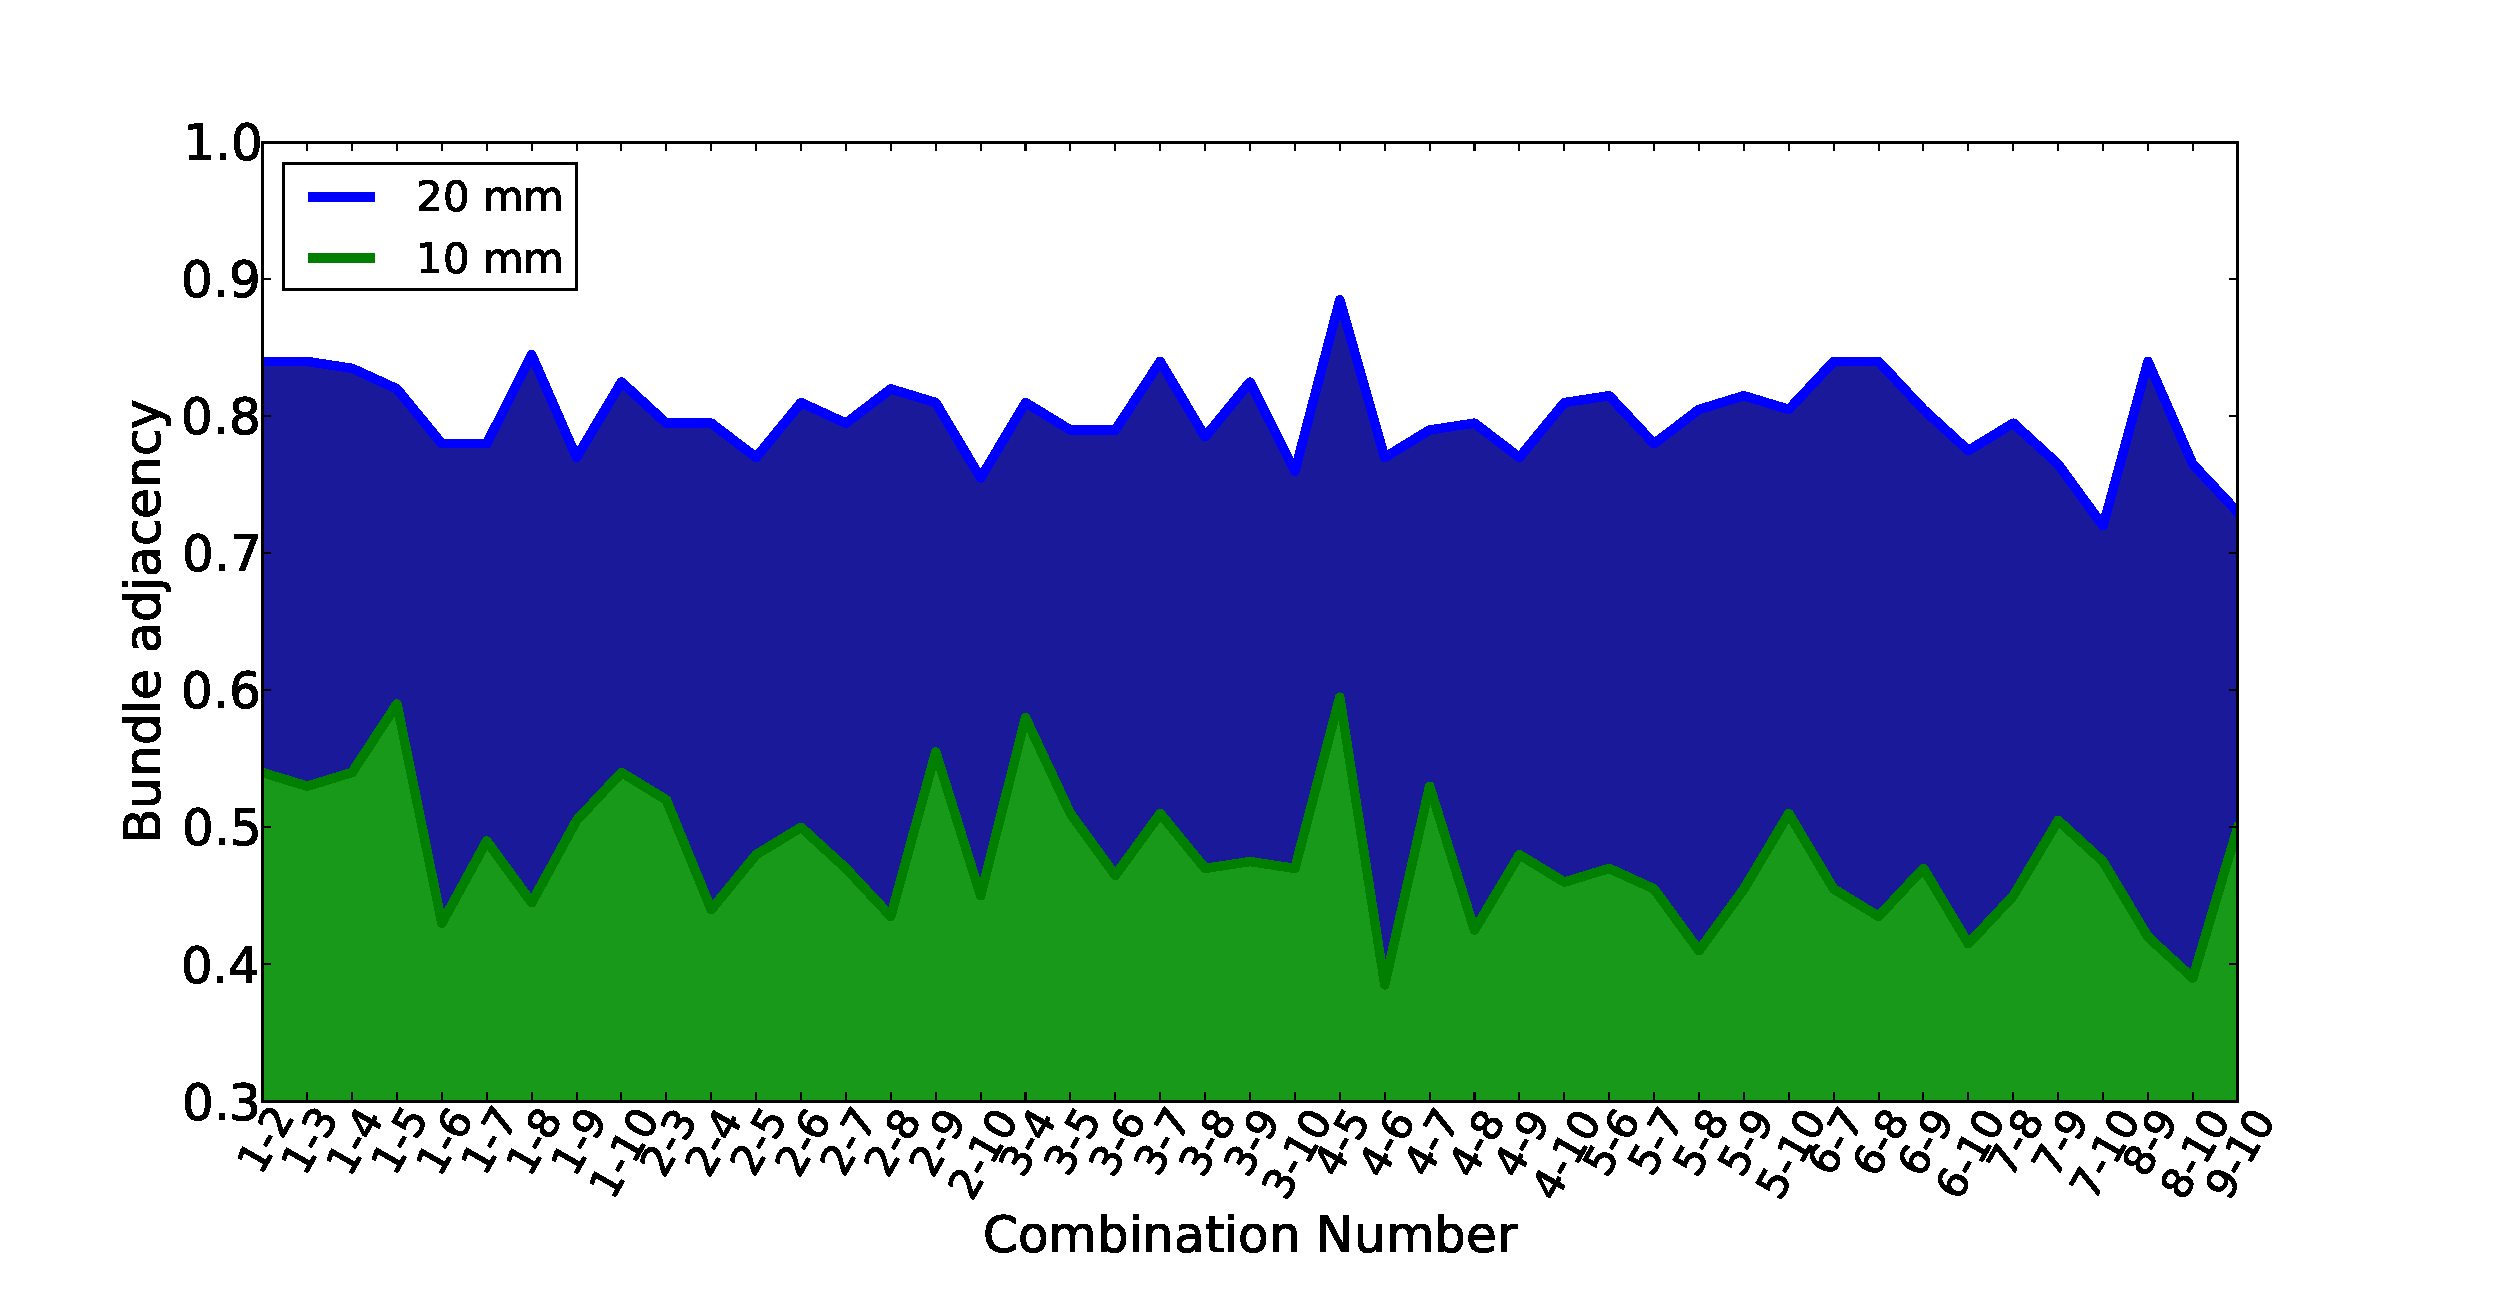
\includegraphics[scale=0.24]{Figures/Fig_13_BAs}}
\caption{Bundle Adjacencies for the 45 pairs of 10 subjects with two
  different distance thresholds. \label{Flo:BAs_plot}}
\end{figure}

For this purpose we evaluated BA (see
section~\ref{sub:Tightness-comparisons-1}) between all pairs of these
$100$ centroids of each of the $10$ tractographies. This generated $45$
BA values with $\theta=10$~mm (BA10). We also generated another $45$ BA
values with $\theta=20$~mm (BA20). It is noticeable here that the
distance threshold for BA is twice that of the initial QB distance
threshold. 
% The results of this experiment are presented in
% Fig.~\ref{Flo:BAs_plot}.

For BA10 the most dissimilar subjects were subjects 4 and 6 with
BA10(4,6)=38.5\%. The most similar subjects were 4 and 5 with
BA10(4,5)=59.5\%. The mean BA10 was 48\% ($\pm\num{4.9}$\%). With
BA20 the most dissimilar subjects were subjects 7 and 10 with
BA20(7,10)=72\%. The most similar subjects were, in agreement with BA10,
4 and 5 with BA20(4,5)=88.5\%. The mean BA20 was 80\%
($\pm\num{3.2}$\%).

In future work we would like to study how the length of the big clusters
affects BA. In this experiment there was a great variability of centroid
lengths (mean $73.6$~mm $\pm\num{43.9}$~mm). If we suppose that shorter
streamlines are more likely to be noise artifacts we would expect that
by concentrating on longer streamlines we would have a more robust
similarity measure for tractography comparison.


\subsection{Limitations of QB\label{sub:short_tracks}}

Usually taking short streamlines into account is not valid because (a)
the longer streamlines are more likely to be used as useful landmarks
when comparing or registering different subjects because it is more
likely for them to be present in most subjects, (b) removing short
streamlines facilitates the usage of distance based clustering (no need
for manually setting the distance threshold) and interaction with the
tractography, (c) typically one first wants to see the overall
representation of the tractography and later go to the details. MDF
distance often separates shorter from longer neighbouring streamlines
which is both a strength and a limitation according to
application. Nonetheless, after having clustered the longer streamlines
there are many ways to assign the shorter clusters to their closest
longer clusters. For this purpose we recommend to use a different
distance from MDF for example the minimum version of MAM referred to as
$\textrm{MAM}_{\textrm{min}}$ in Eq.~(\ref{eq:minimum_distance}).

%
\begin{figure}
  \centerline{\hspace{-1.5mm}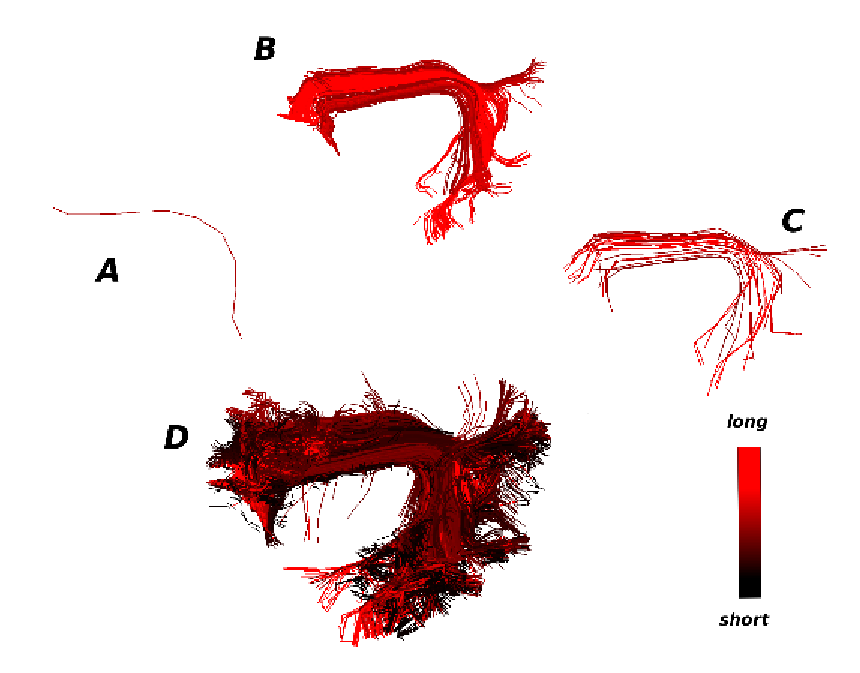
\includegraphics[scale=0.65]{Figures/Fig_10_arcuate_small_fibers}}
  \caption{What could be considered as the strength and limitation of QB
    is that short streamlines will be clustered differently than longer
    streamlines although they may belong in the same anatomical
    bundle. A solution to this problem is illustrated. The colormap here
    encodes streamline length. A: a single centroid streamline, B: the
    $245$ actual streamlines closer than $15$~mm (MDF distance), C: the
    streamlines from B clustered with $23$ centroid streamlines using QB
    with threshold $6.25$~mm, D: the $\num{3421}$ actual streamlines
    closer than $6$~mm ($\textrm{MAM}_{\textrm{min}}$ distance) from the
    centroid streamlines in C are shown. We can see that a great number
    of short streamlines have been brought together along with the
    streamlines in B. \label{Flo:arcuate_close}}
\end{figure}

Here we discuss two simple strategies for clustering short
streamlines. The first is an unsupervised technique and the second is
supervised.

1. Cluster the long streamlines using QB with distance threshold at
$10$~mm and then cluster the short streamlines (<$100$~mm) to a lower
threshold and assign them to their closest long streamline bundle from
the first clustering using the $\mathrm{MAM}_{\mathrm{min}}$ distance.

2. Read and cluster the tractography of a subject, pick a centroid
streamline from that atlas and then find the closest streamlines from
the subject to that selected streamline using MDF, cluster the closest
streamlines found from the previous step and for each one of these new
centroid streamlines find the closest streamlines using the
$\textrm{MAM}_{\textrm{min}}$ distance. We should now have an
amalgamation of shorter and longer streamlines in one cluster.

An example of this second strategy is shown in
Fig.~\ref{Flo:arcuate_close}. A single centroid streamline of interest
(A) from the region of arcuate fasciculus is selected
Fig.~\ref{Flo:arcuate_close}; the streamlines closer than 15~mm (MDF) to
the selected cluster are shown (B) and clustered with a distance
threshold of $6.25$~mm (C); finally from every centroid streamline in C
we find the closest streamlines (D) using the
$\textrm{MAM}_{\textrm{min}}$ distance from the entire tractography. In
this way we managed to bring together in a semi-automatic fashion an
entire bundle consisting both of long and short streamlines by just
selecting initially a single representative streamline.

\section{Discussion and conclusion}

We have presented a novel and powerful algorithm -- QuickBundles
(QB). This algorithm provides simplifications to the old problem of
revealing the detailed anatomy of the densely packed white matter which
has recently attracted much scientific attention; it can also be used
for any trajectory clustering problem and it is recommended when large
data sets are involved. QB can be used with all types of diffusion MRI
tractographies which generate streamlines (e.g. probabilistic or
deterministic) and it is independent of the reconstruction model. QB is
supported by a distance function MDF on the space of streamlines which
makes it a metric space. QB can achieve compression ratios of the order
of 200:1 depending on the distance threshold while preserving
characteristic information about the tractography.

In common with mainstream clustering algorithms such as k-means,
k-centers and expectation maximization, QB is not a global clustering
method therefore it can give different results under different initial
conditions of the data set when there is no obvious distance threshold
which can separate the clusters into meaningful bundles; for example we
should expect different clusters under different permutations/orderings
of the streamlines in a densely packed tractography. However, we found
that there is good agreement even between two clusterings of the same
tractography with different orderings. If the clusters are truly
separable by distances then there is a global solution independent of
orderings. This is often visible in smaller subsets of the initial
tractography. 

Other algorithms previously too slow to be used on the entire
tractography can now be used efficiently too if they start their clustering
on the output of QB rather than the initial full tractography.

We saw that QB is a linear time clustering method based on streamline
distances, which is on average linear time $\mathcal{O}(N)$ where $N$ is
the number of streamlines and with worst case $\mathcal{O}(N^{2})$ when
every streamline is a singleton cluster itself. Therefore QB is the
fastest known tractography clustering method and even real-time on
smaller tractographies ($\le$~\num{20000} streamlines, depending on
system CPU). We also showed that it uses a negligible amount of memory.

QB is fully automatic and very robust as when we use it we can find good
agreements even between different subjects. Additionally, it can be used
to explore multiple tractographies and find correspondences or
similarities between different tractographies. This can be facilitated
by the use of Bundle Adjacency (BA) a new similarity measure introduced
in this paper.

The reduction in dimensionality of the data achieved by QB means that
BOIs (bundles of interest) can be selected as an alternative to ROIs for
interrogating the data. We also showed that QB can be used to find
obscured streamlines not visible to the user at first
instance. Therefore QB opens up the road to create rapid tools for
exploring tractographies of any size.

In the future we would like to investigate different ways to merge QB
clusters by integrating prior information from neuroanatomists. We are
currently working on developing interactive tools which exploit the
simplification that QB provides \citep[see][]{GaryfallidisHBM2012}.

We have shown results with data from simulations, single and multiple
real subjects. The code for QuickBundles is freely available at
$\texttt{dipy.org}$.

\section*{Acknowledgements}
We gratefully acknowledge valuable discussions with Arno Klein and John
Griffiths on various aspects of this work.

\section*{Disclosure/Conflict-of-Interest Statement}
There are no conflicts of interest relating to this work.

\selectlanguage{british}%
\bibliographystyle{apalike2}
%\bibliographystyle{plainnat}
%\bibliographystyle{IEEEabrv, IEEEtran}
%\bibliographystyle{IEEEtran}
%\bibliographystyle{elsarticle-harv}
\selectlanguage{english}
\bibliography{diffusion}

\end{document}
